

	
%\include{Portada3} 	

\chapter{Trabajando con Datos de Texto}\label{Cap7}


\section{Introducción}

En el Capítulo \ref{Cap4}, hablamos sobre dos tipos de características que pueden representar 
propiedades de la data: características continuas que describen una cantidad y características categóricas que son items  de una lista fija. Hay un tercer tipo de característica que se puede encontrar en muchos
aplicaciones,  el tipo  texto.  Por ejemplo, si queremos clasificar un mensaje de correo electrónico como
 un correo electrónico legítimo o spam, el contenido del correo electrónico ciertamente contendrá
información importante para esta tarea de clasificación.  O tal vez queremos aprender sobre la opinión de un político sobre el tema de la inmigración.  En este caso, los discursos o tweets de esta persona pueden proporcionar información útil.   En servicio al cliente, a menudo desea saber si un mensaje es una queja o una consulta.   Podemos usar la línea del tema y contenido de un mensaje para determinar automáticamente la intención del cliente, que nos permite enviar el mensaje al departamento correspondiente, o incluso enviar una  respuesta automática.\\


La data de texto generalmente  suelen representarse como cadenas (strings), compuestas de caracteres. En cualquiera de los ejemplos que se acaban de dar, la longitud de los datos de texto variará. Esta característica es claramente muy diferente de las características numéricas que hemos discutido hasta ahora, y tendremos que procesar los datos antes de que podamos aplicar nuestros algoritmos de aprendizaje automático sobre ellos.\\

% oraciones  críticas    reseñas o críticas comentarios 

\section{Tipos de datos representados como cadenas}

Antes de sumergirnos en los pasos de procesamiento que van en la representación de datos de texto para el aprendizaje automático, queremos discutir brevemente diferentes tipos de datos de texto que se  podría encontrar. El texto suele ser sólo una cadena en la dataset, pero no todas las características de cadena deben tratarse como texto. Una característica de cadena (string) algunas  veces puede representar variables categóricas, como discutimos en el Capítulo \ref{Cap5}. No hay manera de saber cómo tratar una característica de cadena antes de revisar la data.\\


\noindent Hay cuatro tipos de datos de cadena (string) que puede ver:

\begin{list}{$\bullet$}{}  
	
	\item Datos categóricos.
	
	\item  Cadenas libres que pueden asignarse semánticamente a categorías.
	
	\item   Datos de cadena estructurados.
	
	\item  Datos de texto. 
\end{list}Los datos categóricos son los datos  que viene en forma  de una lista fija. Digamos que recopila datos a través de una encuesta donde le preguntas a las personas su color favorito, con un menú desplegable que les permite  seleccionar entre "{}rojo"{}, "{}verde"{}, "{}azul"{}, "{}amarillo"{}, "{}negro"{}, "{}blanco"{}, "{}púrpura"{} y "{}rosa"{}. 
Esto dará como resultado una dataset con exactamente ocho posibles valores  diferentes, que claramente
codifican una variable categórica. Puede verificar  por  observación  si este es el caso de sus datos
(si ve muchas cadenas diferentes, es poco probable que esta sea una variable categórica) y confirmarlo calculando los valores únicos sobre el conjunto de datos, y posiblemente usando un histograma con  la frecuencia con que aparece cada uno. 
También es posible que desee verificar si cada variable corresponde realmente a una categoría que tiene sentido para su aplicación. Tal vez a la mitad de la existencia de su encuesta, alguien descubrió que
"{}negro"{} fue mal escrito como "{}negor"{} y posteriormente corrigió la encuesta. Como resultado, su
la data contiene "{}negor"{} y "{}negro"{}, que corresponden al mismo 
significado  semántico  y debe consolidarse.\\



Ahora imagine que en lugar de proporcionar un menú desplegable, proporciona un campo de texto para que los 
usuarios  proporcionen sus propios colores favoritos. Muchas personas pueden responder con el nombre de un un color, como "{}negro"{} o "{}azul"{}. Otros pueden cometer errores tipográficos, usar diferentes
ortografías como "{}gris"{} y "{}grises"{}, o use nombres más evocadores y específicos como "{}noche azul."{} También tendrás algunas entradas muy extrañas.  Algunos buenos ejemplos vienen
de la encuesta de color xkcd  (\href{https://blog.xkcd.com/2010/05/03/color-survey-results/}{\textcolor{vino}{xkcd Color Survey} }), donde la gente tuvo que nombrar colores y se les ocurrió nombres como "{}velociraptor cloaka"{}    y   "{}El consultorio  naranja de mi dentista.  Todavía recuerdo su  caspa lentamente flotando en mi enorme bostezo"{}; ejemplos como estos,  son difíciles de asignar a colores automáticamente (o en absoluto).   Las respuestas que puede obtener de un campo de texto pertenecen a la segunda categoría en la lista, son  \emph{cadenas libres que pueden asignarse semánticamente a categorías}. 
Estos datos probablemente sea mejor codificarlos  como una variable categórica, donde pueda 
seleccionar las categorías utilizando las entradas más comunes o definiendo categorías que capturen las respuestas de una manera que tenga sentido para su aplicación.  Se podría tener algunas categorías para colores estándar, tal vez una categoría  "{}multicolor"{}   para personas que dieron respuestas como  "{}rayas verdes y rojas"{}  y una   categoría  como  "{}otra"{}  para respuestas que no pueden ser codificadas de otra manera. 
 Este tipo de preprocesamiento de  cadenas pueden requerir mucho esfuerzo manual y no se automatizan fácilmente.  Si estás en una posición que  puede influir en la recopilación de datos, le recomendamos que evite valores introducidos de forma manual para conceptos que se capturan mejor utilizando variables categóricas.\\


Con frecuencia, los valores introducidos manualmente no corresponden a categorías fijas, pero todavía tienen alguna estructura subyacente, como direcciones, nombres de lugares o personas, fechas, números de teléfono o cualquier otro identificador. Este tipo de cadenas son a menudo muy difíciles de analizar, y su tratamiento es altamente dependiente del contexto y el dominio. Un tratamiento sistemático de estos casos está más allá del objetivo de este libro.\\


La categoría final de  datos de cadena son los datos de texto en forma libre (freeform) que consisten en frases o sentencias  (phrases or sentences). Los ejemplos incluyen tweets, registros de chat y reseñas de hoteles, así como las obras recopiladas de Shakespeare, el contenido de Wikipedia o la colección del Proyecto Gutenberg de 50.000 libros electrónicos.


 Todas estas colecciones contienen información principalmente como oraciones compuestas de palabras\footnote{Discutiblemente, el contenido de sitios Webes asociados a tweets contiene más información que el texto de tweets en sí mismos.}. Por simplicidad, asumamos que todos nuestros documentos están en un idioma, inglés\footnote{La mayor parte de lo que hablaremos en el resto del capítulo también se aplica a otros idiomas que usan el alfabeto romano, y parcialmente a otros idiomas con delimitadores de límites de palabras. El chino, por ejemplo, no  delimita los límites de las palabras y tiene otros desafíos que dificultan la aplicación de las técnicas de este capítulo.}. En el contexto del análisis de texto, el conjunto de datos a menudo se llama cuerpo (corpus), y cada punto de datos, representado como un sólo texto, se llama documento. Estos términos provienen de la comunidad de recuperación de información (IR) y procesamiento del lenguaje natural (PNL), ambos  se ocupan principalmente de datos de texto.

 
\subsection{Ejemplo de aplicación:  Análisis de Sentimiento a Comentarios de Película}
   
  
%   the information retrieval (IR) and natural language processing (NLP) community, \\
%    reviews comentarios reseñas\\

Como ejemplo en ejecución en este capítulo, usaremos una dataset de reseñas o comentarios de películas
 del sitio web de IMDb (Internet Movie Database) recopilados por el investigador de   Stanford Andrew Maas\footnote{La data está disponible en   
 \href{http://ai.stanford.edu/~amaas/data/sentiment/}{\color{vino} http://ai.stanford.edu/~amaas/data/sentiment/}.}.   Esta dataset  contiene el texto de los comentario, junto con una etiqueta que indica si un  comentario es "{}positivo"{}  o  "{}negativo."{}   El sitio web de IMDb contiene clasificaciones de 1 a 10. Para simplificar el modelado, esta anotación se resume como una  dataset de clasificación en dos clases, donde los comentarios con una puntuación igual o superior a 6 se etiquetan como positivos, y el resto como negativos. Se deja  la pregunta de si esta es una buena representación de los datos abiertos si mayor análisis, y simplemente usaremos la data según lo proporcionado por Andrew Maas.\\

Después de descomprimir los datos, se obtienen los archivos de texto  en dos carpetas separadas, una con los datos de entrenamiento y otra con los datos de prueba. Cada uno de estos a su vez tiene dos subcarpetas, una llamada  {\ttfamily pos} y otra llamada {\ttfamily neg} :

\begin{lstlisting}

In[2]:

   !tree -L 2 C:/Data/aclImdb_v1/aclImdb

Out[2]:

\end{lstlisting}
\vspace{-0.6cm}
\begin{figure}[h!]
	%\centering
	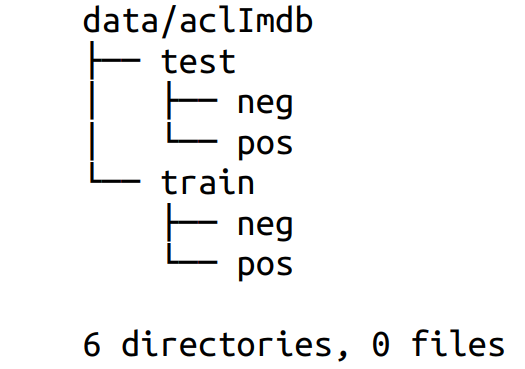
\includegraphics[scale=0.35]{Imagen_Machine/Texto1}
%	\caption{Matriz de confusión para clasificación binaria}
%	\label{Pipe3}
\end{figure}

La carpeta  {\ttfamily pos} contiene todas las críticas positivas, cada una como un archivo de texto separado, y similarmente  en  la carpeta  {\ttfamily neg}. 

Hay una función auxiliar en  {\ttfamily scikit-learn}  para cargar archivos almacenados con tal estructura de carpetas, donde cada subcarpeta corresponde a una etiqueta, llamada  {\ttfamily load\_files.} 
Aplicamos la función  {\ttfamily load\_files } primero a los datos de entrenamiento:
 
%   reviews_train = load_files("C:/A Cuadernos De Python/aclImdb_v1/aclImdb/train/")


\begin{lstlisting}

In[3]:

   # Descargue la data aqui:    (Archivo comprimido)
   #      http://ai.stanford.edu/~amaas/data/sentiment/aclImdb_v1.tar.gz
   
   # Mi direcccion es:   C:\Data\aclImdb_v1\aclImdb
   # Puede tardar 10 minutos o mas, paciencia
   
   from sklearn.datasets import load_files
   
   reviews_train = load_files("C:/Data/aclImdb_v1/aclImdb/train/")

  
   # load_files returns a bunch, containing training texts and 
   # training labels
   text_train, y_train = reviews_train.data, reviews_train.target
   print("type of text_train: {}".format(type(text_train)))
   print("length of text_train: {}".format(len(text_train)))
   print("text_train[1]:\n{}".format(text_train[1]))
  
Out[3]:

   type of text_train: <class 'list'>
   length of text_train: 25000
   text_train[1]:
   b'Words can\'t describe how bad this movie is. I can\'t explain it by
     writing only. You have too see it for yourself to get at grip of how 
     horrible a movie really can be. Not that I recommend you to do that. 
     There are so many clich\xc3\xa9s, mistakes (and all other negative 
     things you can imagine) here that will just make you cry. To start with 
     the technical first, there are a LOT of mistakes regarding the airplane.
     I won\'t list them here, but just mention the coloring of the plane. 
     They didn\'t even manage to show an  airliner in the colors of a 
     fictional airline, but instead used a 747 painted in the original 
     Boeing livery.  Very bad. The plot is stupid and has been done many 
     times before, only much, much better. There are so many ridiculous
     moments here that i lost count  of it really early. Also, I was on the
     bad guys\' side all the time in the movie, because the good guys were 
     so stupid. "Executive Decision" should without a doubt be you\'re choice
     over this one, even the "Turbulence"-movies are better. In fact, every
     other movie in the world is better than this one.'

\end{lstlisting}

% b'Las palabras no pueden describir lo mala que es esta película. No puedo explicarlo por escribiendo solamente. Tienes que verlo por ti mismo para saber cómo una película realmente horrible puede ser. No es que te recomiendo que hagas eso. Hay tantos clichés \ xc3 \ xa9s, errores (y todos los demás cosas que puedas imaginar) aquí que te harán llorar. Para empezar lo técnico primero, hay MUCHOS errores con respecto al avión.  No los enumeraré aquí, pero solo mencionaré el color del avión. Ni siquiera lograron mostrar un avión con los colores de un aerolínea ficticia, pero en su lugar usó un 747 pintado en el Boeing original  librea. Muy mal. La trama es estúpida y se ha hecho muchas veces antes,  solo que mucho, mucho mejor. Hay tantos momentos ridículos aquí que yo  Perdí la cuenta muy temprano. Además, estaba del lado de los malos todos el tiempo en la película, porque los buenos eran tan estúpidos. "Ejecutivo  La decisión "debe ser sin duda su elección sobre esta, incluso las películas de "Turbulencia" son mejores. De hecho, todas las demás películas del el mundo es mejor que este '.







Puedes ver que {\ttfamily text\_train} es una lista de longitud 25.000, donde cada entrada es una cadena que contiene una crítica o comentario. Imprimimos la reseña con el índice 1. También puede ver que la reseña contiene algunos saltos de línea HTML (<br />, breaks). Si bien es poco probable que estos tengan un gran impacto en nuestros modelos de aprendizaje automático, es mejor limpiar los datos y eliminar este formato antes de proceder:

\begin{lstlisting}%[frame=single]

In[4]:

   text_train = [doc.replace(b"<br />", b" ") for doc in text_train]

\end{lstlisting}


El tipo de  entrada de {\ttfamily text\_train} dependerá de la versión de Python. En Python 3, serán de tipo bytes  que representa una codificación binaria de los datos de cadena (strings). En Python 2, el {\ttfamily text\_train} contiene cadenas. Aquí, no entraremos en los detalles de los diferentes tipos de cadenas en Python, pero te recomendamos que leas la documentación de \href{https://docs.python.org/2/howto/unicode.html}{\textcolor{vino}{ Python 2} }  y/o  \href{https://docs.python.org/3/howto/unicode.html}{\textcolor{vino}{ de Python 3} } sobre cadenas y Unicode.\\

La dataset se recogió de tal manera que la clase positiva y la clase negativa sean balanceadas, de modo que hay tantas cadenas (string) positivas como negativas: 


\begin{lstlisting}%[frame=single]

In[5]:

   print("Samples per class (training): {}".format(np.bincount(y_train)))

Out[5]:
 
   Samples per class (training): [12500 12500] 
 \end{lstlisting}  
   
     Cargamos la dataset de prueba en la misma forma:
     
\begin{lstlisting}%[frame=single]

In[6]:

     
   reviews_test = load_files("C:Data/aclImdb_v1/aclImdb/test/") 
      
   text_test, y_test = reviews_test.data, reviews_test.target
   print("Number of documents in test data: {}".format(len(text_test)))
   print("Samples per class (test): {}".format(np.bincount(y_test)))
   text_test = [doc.replace(b"<br />", b" ") for doc in text_test]

Out[6]:

   Number of documents in test data: 25000
   Samples per class (test): [12500 12500]

\end{lstlisting}

La tarea que queremos resolver es la siguiente: dada una reseña o comentario, queremos 
asignarle una etiqueta  "{}positivo"{}  o  "{}negativo."{} basada en el contexto del comentario o 
reseña. Esta es una tarea de clasificación binaria estándar. Sin embargo, la data de texto
no está en formato para que el modelo de aprendizaje automatico pueda manejarlo.
Necesitamos convertir la representación de  cadenas (string) de texto  en representación 
numérica que pueda aplicarle el algoritmo de aprendizaje automático.

\subsection{Representando la data de texto en bolsas de palabras}

%  Representing Text Data as a Bag of Words}
%  palabras que no aportan información relevante sobre el texto. Ha estas palabras se les conoce como stopwords.
 
Una de las maneras más simples pero efectivas y comúnmente utilizadas para representar el texto para el aprendizaje automático es usando  la representación de la bolsa de palabras (del inglés, Bag of Words)\footnote{El modelo "bolsa de palabras" (del inglés, Bag of Words) es un método que se utiliza en el procesado del lenguaje para representar documentos ignorando el orden de las palabras. En este modelo, cada documento parece una bolsa que contiene algunas palabras. Por lo tanto, este método permite un modelado de las palabras basado en diccionarios, donde cada bolsa contiene unas cuantas palabras del diccionario.}. Al usar esta representación, descartamos la mayor parte de la estructura del texto de entrada, como capítulos, párrafos, oraciones y formatos, y sólo contamos {\emph{la frecuencia con la que cada palabra aparece en cada texto}}  del cuerpo.

 Descartando la estructura y contando sólo las ocurrencias de palabras conduce a la imagen mental de representar el texto como una "{}bolsa."{}  \\
 
  El cálculo de la representación de la bolsa de palabras para un cuerpo (corpus) de documentos consta de los tres pasos siguientes:
  
\begin{enumerate}
	
	\item \emph{Tokenización}. Dividir cada documento en las palabras que aparecen en él (llamadas tokens), por ejemplo, dividiéndolos en espacios en blanco y puntuación.
	
	\item \emph{La construcción de vocabulario}. Recoger un vocabulario de todas las palabras que aparecen en cualquiera de los documentos, y el número de ellos (por ejemplo, en orden alfabético). 
	
	\item \emph{Codificación}. Para cada documento, se cuenta la frecuencia   con   que  aparece cada palabras del vocabulario en este documento.
	
\end{enumerate}

Hay algunas sutilezas involucradas en los pasos 1 y 2, que discutiremos   más adelante con más detalle  en este capítulo. Por ahora, veamos cómo podemos aplicar el procesamiento de la bolsa de palabras usando {\ttfamily scikit-learn}. En la Figura \ref{Texto2} se ilustra el proceso en la cadena "{}Así es como se obtienen las hormigas{}". La salida es un vector de recuento de palabras para cada documento. 
Para cada palabra en el vocabulario, tenemos un recuento de la frecuencia con que aparece en cada documento. Eso significa que nuestra representación numérica tiene una característica para cada palabra única en toda la data. Observe cómo el orden de las palabras en la cadena original es completamente irrelevante para la representación de la función bag-of-words.

\begin{figure}[h!]
	\centering
	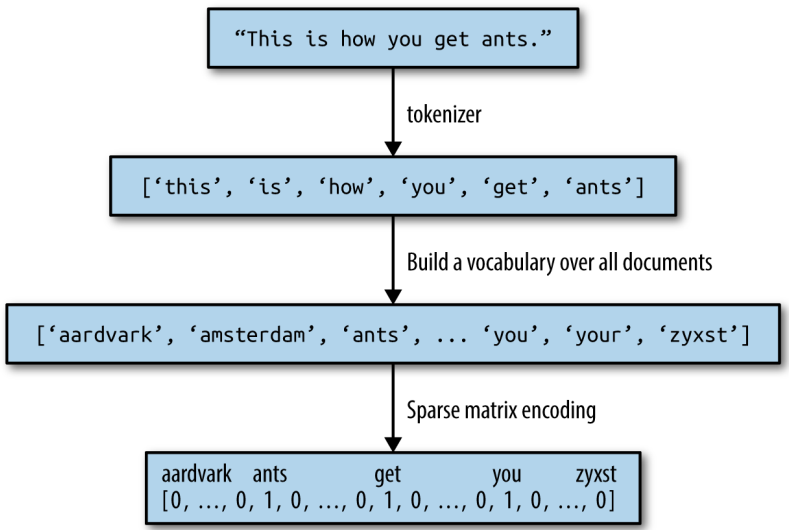
\includegraphics[scale=0.65]{Imagen_Machine/Texto2}
	\caption{Procesamiento de bolsa de palabras (bag-of-words)}
	\label{Texto2}
\end{figure}



\subsection{Aplicando Bag-of-Words en la dataset Toy}


La representación de la bolsa de palabras se implementa en {\ttfamily CountVectorizer}, que es un transformador. Para ver como  funciona lo aplicaremos sobre la  dataset Toy, que consta de dos muestras:

\begin{lstlisting}%[frame=single]

In[7]:
   
   bards_words =["The fool doth think he is wise,",
                 "but the wise man knows himself to be a fool"]
 
 \end{lstlisting}
 
 Importamos e instanciamos al {\ttfamily CountVectorizer} y ajustamos en la data Toy como sigue:
 
 \begin{lstlisting}%[frame=single]
 
  
In[8]:

   from sklearn.feature_extraction.text import CountVectorizer
   vect = CountVectorizer()
   vect.fit(bards_words)
   
    \end{lstlisting}
   
  El ajuste de {\ttfamily CountVectorizer} consiste en la tokenización de los datos de entrenamiento y la
  construcción del vocabulario, al que podemos acceder como el atributo {\ttfamily vocabulary\_}: 
   
   \begin{lstlisting}%[frame=single]
   
In[9]:

   print("Vocabulary size: {}".format(len(vect.vocabulary_)))
   print("Vocabulary content:\n {}".format(vect.vocabulary_))

Out[9]:

   Vocabulary size: 13
   Vocabulary content:
    {'the': 9, 'himself': 5, 'wise': 12, 'he': 4, 'doth': 2, 'to': 11, 
     'knows': 7,  'man': 8, 'fool': 3, 'is': 6, 'be': 0, 'think': 10,
     'but': 1}
   
    \end{lstlisting}
  
  El vocabulario consta de 13 palabras, desde "{}ser"{} ("{}be"{})  hasta "{}sabio"{} ("{}wise"{}). \\
  
  Para crear la representación de bolsa de palabras para los datos de entrenamiento, llamamos al método transformación   {\ttfamily transform:}  

 \begin{lstlisting}%[frame=single]

In[10]:

   bag_of_words = vect.transform(bards_words)
   print("bag_of_words: {}".format(repr(bag_of_words)))

Out[10]:

   bag_of_words: <2x13 sparse matrix of type '<class 'numpy.int64'>'
       with 16 stored elements in Compressed Sparse Row format>

\end{lstlisting}

La representación de la bolsa de palabrs (bag-of-words) se almacena en una matriz sparse de
SciPy que sólo almacena las entradas que no son cero (ver Capítulo \ref{Cap1} ). La matriz es de 
forma 2x13, con una fila para cada uno de los dos puntos de datos y una característica para
cada una de las palabras  del vocabulario.  
Se utiliza una matriz sparse (dispersa) ya que la  mayoría de los documentos sólo contienen un
 pequeño subconjunto de las palabras en el vocabulario, lo que significa que la mayoría de las  entradas en la matriz de características son 0.  Piense en cuántas palabras diferentes pueden aparecer en un comentario  de una película en comparación con todas las palabras en el idioma inglés (que es lo que modela el vocabulario).

Almacenar todos esos ceros sería improductivo, y un desperdicio de memoria. Para observar el
 contexto real de la matriz sparse, podemos convertirla en una matriz NumPy  "{}densa"{} 
(que también almacena todas las entradas 0) usando el método  {\ttfamily toarray}\footnote{Esto es posible porque estamos utilizando un data pequeña, Toy que contiene sólo 13 palabras. Para cualquier conjunto de datos real, esto daría lugar a un {\ttfamily MemoryError}.}:


\begin{lstlisting}%[frame=single]

In[11]:

   print("Dense representation of bag_of_words:\n{}".format(
          bag_of_words.toarray()))

Out[11]:

   Dense representation of bag_of_words:
   [[0 0 1 1 1 0 1 0 0 1 1 0 1]
    [1 1 0 1 0 1 0 1 1 1 0 1 1]]

\end{lstlisting}


Podemos ver que los recuentos de palabras para cada palabra son 0 o 1; ninguna de las dos cadenas en {\ttfamily bards\_words} contiene una palabra dos veces.

Echemos un vistazo a cómo leer estos vectores de características. La primera cadena ("{}El necio piensa que es sabio{}") ("{}The fool doth think he is wise"{})  se representa como la primera fila, y contiene la primera palabra en el vocabulario, "{}ser"{} ("{}be"{}), cero veces. También contiene la segunda palabra en el vocabulario, "{}pero"{} ("{}but"{}), cero veces. Contiene la tercera palabra, "{}doth"{}, una vez, y así sucesivamente. Observando ambas filas, podemos ver que la cuarta palabra, "{}tonto"{} ("{}fool"{}), la décima palabra, "{}el"{}  ("{}the"{}), y la decimotercera palabra, "{}sabio"{} ( "{}wise"{}), aparecen en ambas cadenas.

\subsubsection{Bolsa de palabras para las críticas de cine}

% Bag-of-Words for Movie Reviews

Ahora que hemos pasado por el proceso de la bolsa de palabras en detalle, vamos a aplicarlo 
a la tarea de análisis de sentimientos para las críticas de cine. Anteriormente, hemos
 cargado la data de entrenamiento y pruebas de las reseñas de IMDb en listas de cadenas 
 ({\ttfamily text\_train}  y  {\ttfamily  text\_test}), que ahora procesaremos:


\begin{lstlisting}%[frame=single]

In[12]:

   vect = CountVectorizer().fit(text_train)
   X_train = vect.transform(text_train)
   print("X_train:\n{}".format(repr(X_train)))

Out[12]:

   X_train:
   <25000x74849 sparse matrix of type '<class 'numpy.int64'>'
       with 3431196 stored elements in Compressed Sparse Row format>

\end{lstlisting}

La forma de {\ttfamily X\_train}, en la representación de la bolsa de palabras de los datos 
de entrenamiento, es de 25.000x74.849, lo que indica que el vocabulario contiene 74.849 
entradas. De nuevo, los datos se almacenan como una matriz sparse  SciPy. Echemos un 
vistazo al vocabulario con un poco más de detalle. Otra forma de acceder al vocabulario es 
utilizando el método {\ttfamily get\_feature\_name} del vectorizador, que devuelve una lista conveniente 
donde cada entrada corresponde a una característica: 


\begin{lstlisting}%[frame=single]

In[13]:

   feature_names = vect.get_feature_names()
   print("Number of features: {}".format(len(feature_names)))
   print("First 20 features:\n{}".format(feature_names[:20]))
   print("Features 20010 to 20030:\n{}".format(feature_names[20010:20030]))
   print("Every 2000th feature:\n{}".format(feature_names[::2000]))

Out[13]:

\end{lstlisting}

\vspace{-0.6cm}
\begin{figure}[h!]
%	\centering
	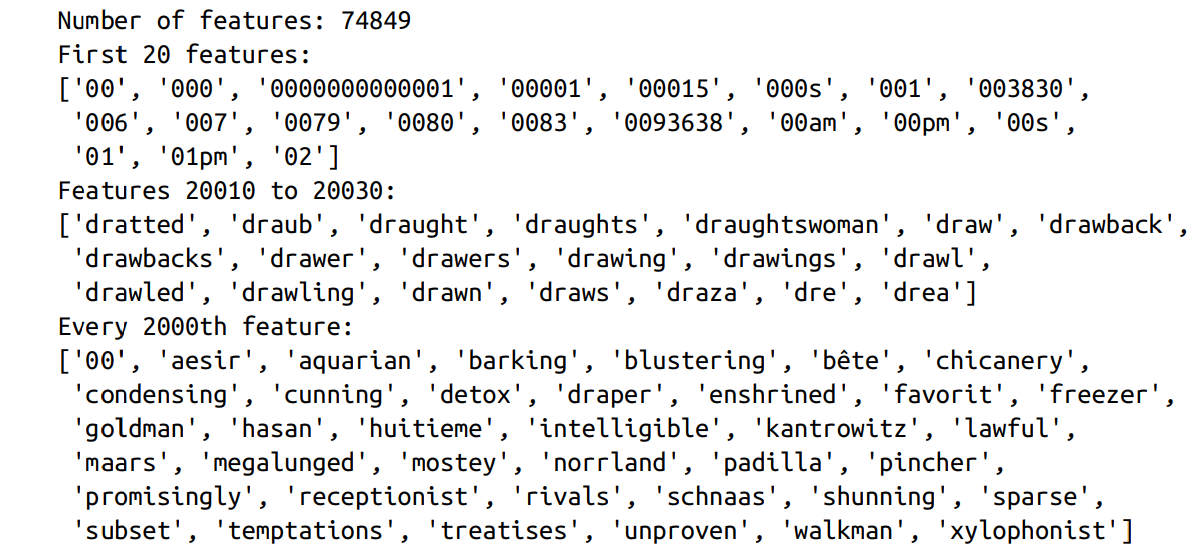
\includegraphics[scale=0.5]{Imagen_Machine/Out13}
%	\caption{Procesamiento de bolsa de palabras (bag-of-words)}
%	\label{Out13}
\end{figure}

Como puede ver, posiblemente un poco sorprendente, las primeras 10 entradas en el vocabulario son todas
números.   Todos estos números aparecen en algún lugar de las reseñas o comentarios,  y  por lo tanto, son
extraído como palabras. La mayoría de estos números no tienen ningún significado semántico inmediato: aparte de "007", que en el contexto particular de las películas es  probable que se refiera a  el personaje de James Bond\footnote{Un análisis rápido de los datos confirma que este es el caso. Intente confirmarlo usted.}. Eliminar lo significativo de las "{}palabras"{} no significativas es a veces difícil. Mirando más allá en el vocabulario,  encontramos una colección de palabras en inglés que comienzan con  con  "{}dra"{}. Puede notar que para  "{}draught, "{}drawback"{}, y  "{}drawer"  \: tanto la forma singular como la plural están contenidas en el  vocabulario como palabras distintas.  Estas palabras tienen significados semánticos estrechamente relacionados, y contarlos como diferentes palabras, correspondientes a diferentes características, podría no ser lo ideal.

%  "{}draught"{} ("{}borrador calado   redacto"{}),  "{}drawback"{} ("{}inconveniente"{}) y "{}drawback"{},  y "{}drawer"  ( "{}cajón"{} gaveta )
 

Antes de tratar de mejorar nuestra extracción de características, vamos a obtener una medida cuantitativa de rendimiento mediante la construcción de un clasificador. Tenemos las etiquetas de entrenamiento almacenadas en {\ttfamily y\_train}, y la representación de la bolsa de palabras de los datos de entrenamiento en {\ttfamily X\_train} para que podamos entrenar a un clasificador sobre estos datos. 
 Para datos de alta dimensión y sparse como este, los modelos lineales como {\ttfamily LogisticRegression} a menudo funcionan mejor.\\
 
Comencemos evaluando {\ttfamily LogisticRegresssion} usando validación cruzada\footnote{Usando la configuración predeterminada de {\ttfamily  CountVectorizer}, en realidad no recoge ninguna estadística, por lo que nuestros resultados son válidos. Usar Pipeline desde el principio sería una mejor opción para aplicaciones, pero lo diferimos para facilitar la exposición.}:


\begin{lstlisting}%[frame=single]

In[14]:

   from sklearn.model_selection import cross_val_score
   from sklearn.linear_model import LogisticRegression
   scores = cross_val_score(LogisticRegression(), X_train, y_train, cv=5)
   print("Mean cross-validation accuracy: {:.2f}".format(np.mean(scores)))

Out[14]:
    
    Mean cross-validation accuracy: 0.88
    
\end{lstlisting}

Obtenemos una puntuación media de validación cruzada del 88\%,  lo que indica un rendimiento 
razonable para una tarea de clasificación binaria balanceada. Sabemos que {\ttfamily LogisticRegression} 
tiene un parámetro de regularización C, que podemos ajustar mediante validación cruzada:

\begin{lstlisting}%[frame=single]

In[15]:

   from sklearn.model_selection import GridSearchCV
   param_grid = {'C': [0.001, 0.01, 0.1, 1, 10]}
   grid = GridSearchCV(LogisticRegression(), param_grid, cv=5)
   grid.fit(X_train, y_train)
   print("Best cross-validation score: {:.2f}".format(grid.best_score_))
   print("Best parameters: ", grid.best_params_)

Out[15]:
   
   Best cross-validation score: 0.89
   Best parameters: {'C': 0.1}

\end{lstlisting}

Obtenemos una puntuación de validación cruzada del 89\% utilizando $C = 0,1$. 
Ahora podemos evaluar la generalización del rendimiento de este ajuste de parámetro en el conjunto de prueba:


\begin{lstlisting}%[frame=single]

In[16]:

   X_test = vect.transform(text_test)
   print("{:.2f}".format(grid.score(X_test, y_test)))

Out[16]:

   0.88

\end{lstlisting}

Ahora, veamos si podemos mejorar la extracción de palabras.  Con la función  {\ttfamily CountVectorizer}
se extrae el tokens usando una expresión regular. Por defecto, la expresión regular que 
se usa es "{}$\setminus$b$\setminus$w$\setminus$w+$\setminus$b"{}.  
Si no está familiarizado con las expresiones regulares, esto significa que
busca todas las secuencias de caracteres que consisten  al menos dos letras o 
números ($\setminus$w) y que están separados por fonteras de palabras (word boundaries) ($\setminus$b). 
No encuentra palabras de una letra, y divide las contracciones como  “doesn’t{}”  o 
  “bit.ly{}”,  pero coincide  con "{}h8ter"{} como una sóla palabra,


 El {\ttfamily CountVectorizer} convierte todas las palabras en caracteres  minúscula, de modo que
“Soon”, “Soon” y “sOon” corresponden al mismo token (y, por lo tanto, la misma característica).
Este mecanismo simple funcionamuy bien en la práctica, pero como vimos anteriormente, obtenemos
muchas características no informativas (como los números). 

Una forma de reducir esto es  usar sólo tokens que aparezcan  al menos en dos documentos (o al menos en cinco documentos, y así sucesivamente). Un token que aparezca en un solo documento  es \emph{poco probable} que aparezca en el conjunto de pruebas y por lo tanto no es útil. Podemos configurar el número mínimo de documentos en un token debe aparecer con el parámetro {\ttfamily min\_df}:

\begin{lstlisting}%[frame=single]

In[17]:

   vect = CountVectorizer(min_df=5).fit(text_train)
   X_train = vect.transform(text_train)
   print("X_train with min_df:\n{}".format(repr(X_train)))

Out[17]:

   X_train with min_df:
    <25000x27271 sparse matrix of type '<class 'numpy.int64'>'
       with 3354014 stored elements in Compressed Sparse Row format>

\end{lstlisting}

Al requerir al menos cinco apariciones de cada token, podemos reducir el número de características a 27.271, como se ve en la salida anterior, sólo alrededor de un tercio de las características originales. Veamos algunas tokens de nuevo:

\begin{lstlisting}%[frame=single]

In[18]:

   feature_names = vect.get_feature_names()
   print("First 50 features:\n{}".format(feature_names[:50]))
   print("Features 20010 to 20030:\n{}".format(feature_names[20010:20030]))
   print("Every 700th feature:\n{}".format(feature_names[::700]))

Out[18]:
\end{lstlisting}

\vspace{-0.6cm}
\begin{figure}[h!]
	%\centering
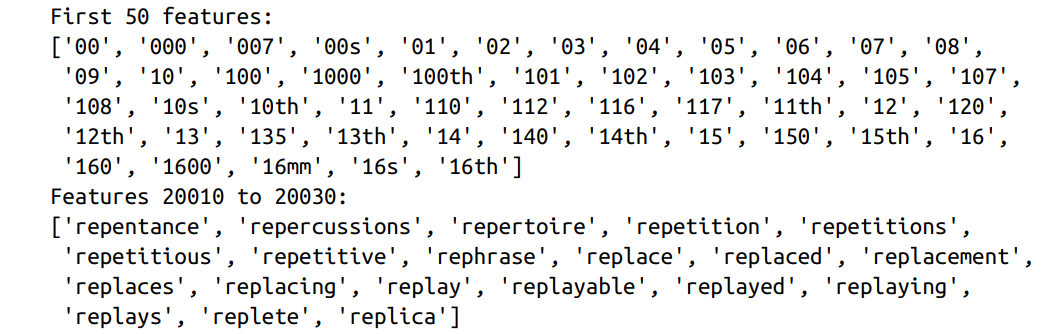
\includegraphics[scale=0.55]{Imagen_Machine/Out18a}
	%	\caption{Matriz de confusión para clasificación binaria}
	%	\label{Pipe3}
\end{figure}

\vspace{-0.9cm}
\begin{figure}[h!]
	%	\centering
	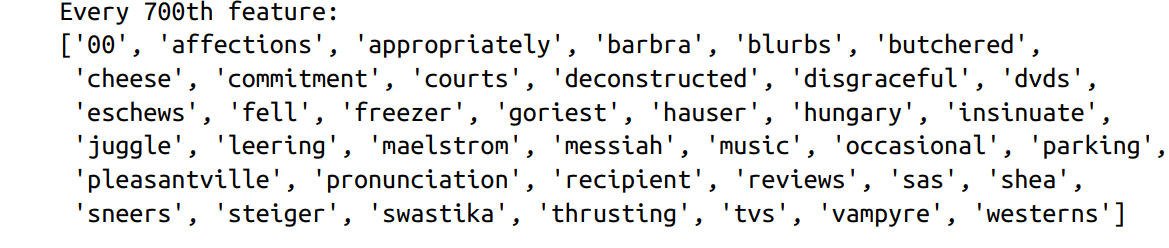
\includegraphics[scale=0.51]{Imagen_Machine/Out18b}
	%	\caption{Procesamiento de bolsa de palabras (bag-of-words)}
	%	\label{Out13}
\end{figure}

Claramente hay muchos menos números, y algunas de las palabras más oscuras o errores ortográficos
parecen haber desaparecido. Veamos qué tan bien funciona nuestro modelo repitiendo  una 
búsqueda por cuadrícula:


\begin{lstlisting}%[frame=single]

In[19]:

   grid = GridSearchCV(LogisticRegression(), param_grid, cv=5)
   grid.fit(X_train, y_train)
   print("Best cross-validation score: {:.2f}".format(grid.best_score_))

Out[19]:
   
   Best cross-validation score: 0.89

\end{lstlisting}

La mejor precisión de validación de la búsqueda en cuadrícula sigue siendo del 89\%, sin cambios desde antes. No mejoramos nuestro modelo, pero tener menos características para hacer frente a las velocidades de procesamiento y desechar características inútiles podría hacer el modelo más interpretable.\\

\begin{minipage}[t]{0.2\textwidth}
	\centering\raisebox{\dimexpr \topskip-\height}{%
		
\includegraphics[width=\textwidth]{Imagen_Machine/Pajaro}}
\end{minipage}%\hfill
\begin{minipage}[t]{0.75\textwidth} 
	{\scriptsize 		
		Si el método de transformación  {\ttfamily CountVectorizer} es llamado en un documento que 
		contiene palabras que no estaban contenidas en los datos de entrenamiento, esas palabras 
		serán ignoradas ya que no son parte del diccionario. Esto no es realmente un problema de clasificación, ya que no es posible aprender nada acerca de las palabras que no están en 
		los datos de entrenamiento. Para algunas aplicaciones, como la detección de spam, podría 
		ser útil añadir una característica que codifica cuántas palabras llamadas \:  "{}fuera de vocabulario"{} \: hay en un documento en particular. Para que esto funcione, es necesario establecer el mínimo con  {\ttfamily min\_df}; de lo contrario, esta característica nunca será activa durante el entrenamiento}
\end{minipage}\\


\subsection{Palabras vacías o Stopwords}

Otra forma para deshacernos de las palabras que no aportan información relevante
sobre el texto, conociadas como Stopwords\footnote{Las palabras que no aportan información relevante sobre el texto, se les conoce como Stopwords, o palabras vacías.}, consiste en desechar las palabras  que son demasiado frecuentes para ser informativas.  Hay dos enfoques principales: usar una lista específica de palabras clave, o descartar palabras que aparecen  con demasiada frecuencia.

 {\ttfamily scikit-learn} tiene una lista integrada de palabras  clave en inglés  en el módulo {\ttfamily feature\_extraction.text}:


\begin{lstlisting}%[frame=single]

In[20]:

   from sklearn.feature_extraction.text import ENGLISH_STOP_WORDS
   print("Number of stop words: {}".format(len(ENGLISH_STOP_WORDS)))
   print("Every 10th stopword:\n{}".format(list(ENGLISH_STOP_WORDS)[::10]))

Out[20]:

   Number of stop words: 318
   Every 10th stopword:
   ['above', 'elsewhere', 'into', 'well', 'rather', 'fifteen', 'had',
    'enough','herein', 'should', 'third', 'although', 'more', 'this',
    'none', 'seemed', 'nobody', 'seems', 'he', 'also', 'fill', 'anyone',
    'anything', 'me', 'the','yet', 'go', 'seeming', 'front','beforehand', 
    'forty', 'i']

\end{lstlisting}


Claramente, eliminando  las palabras  stopwords  en la lista sólo puede disminuir el número de 
características por la longitud de la lista 318, pero podría conducir a una 
mejora en el rendimiento. Veamos una  prueba:

\begin{lstlisting}

In[21]:

   # Specifying stop_words="english" uses the built-in list.
   # We could also augment it and pass our own.
   vect = CountVectorizer(min_df=5, stop_words="english").fit(text_train)
   X_train = vect.transform(text_train)
   print("X_train with stop words:\n{}".format(repr(X_train)))

Out[21]:

   X_train with stop words:
   <25000x26966 sparse matrix of type '<class 'numpy.int64'>'
       with 2149958 stored elements in Compressed Sparse Row format>

\end{lstlisting}

Ahora hay 305 (27.271-26.966) características menos en el conjunto de datos, lo que significa que la mayoría, pero no todas las palabras vacías (stopwords)  aparecieron. Vamos a ejecutar la búsqueda de cuadrícula 
(grid search)  nuevamente:  % appeared

\begin{lstlisting}%[frame=single]


In[22]:

   grid = GridSearchCV(LogisticRegression(), param_grid, cv=5)
   grid.fit(X_train, y_train)
   print("Best cross-validation score: {:.2f}".format(grid.best_score_))

Out[22]:

   Best cross-validation score: 0.88
\end{lstlisting}


El rendimiento de la búsqueda de cuadrícula disminuyó ligeramente usando  stopwords, no lo suficiente como para preocuparse, pero dado que excluir 305 características de más de 27.000 es poco probable que cambie mucho el rendimiento o la interpretabilidad, no parece que valga la pena usar esta lista. 

Las listas fijas son mayormente útiles para conjuntos de datos pequeños, que podrían no contener suficiente información para que el modelo determine qué palabras que son stopwords de los datos mismos. 
Como ejercicio, puede probar el otro enfoque, descartando palabras que aparecen con frecuencia, configurando la opción  {\ttfamily  max\_df}  de {\ttfamily CountVectorizer} y ver cómo influye en el número de características y el rendimiento.



\subsubsection{Re-escalando la data con {\ttfamily \bf{tf–idf}}}
%Rescaling the Data with tf–idf
% Reescalando los datos con tf – idf


En lugar de eliminar características que no se consideran importantes, otro enfoque es
reescalar las características según el nivel de información que esperamos que tengan.
Uno de los  formas más comunes de hacerlo es usado  el  método \emph{term frequency–inverse document frequency}  (tf-idf). 
La intuición de este método es dar mayor peso a cualquier término que aparezca
a menudo en un documento en particular, pero no en muchos documentos  del  corpus.
 Si una palabra aparece con frecuencia  en un documento en particular, pero no en muchos documentos, es probable que sea  muy descriptiva del contenido de ese documento. 
 {\ttfamily scikit-learn} implementa el método {\ttfamily tf–idf}  en dos clases:
  {\ttfamily TfidfTransformer}, que toma la matriz sparse de salida producida por 
   {\ttfamily CountVectorizer}  y los  transforma, y el {\ttfamily TfidfVectorizer}, 
 que toma la data  de texto y realiza tanto la extracción de características
 de bolsa de palabras como la   transformación {\ttfamily  tf–idf.}
  Hay algunas variantes  del esquema de reescalado  de  tf–df, sobre el cual  \href{https://en.wikipedia.org/wiki/Tf-idf}{\textcolor{vino}{puedes leer en Wikipedia} }.   

La puntuación  tf–idf   para la palabra \emph{w} en el documento  d
tal como se implementa en las clases {\ttfamily TfidfTransformer}  y  {\ttfamily TfidfVectorizer}   está dado por{\footnote{\scriptsize{Proporcionamos esta fórmula aquí principalmente para completar; pero no se necesita recordarla para usar la codificación tf-idf}}}:\\
 

 $ tfidf(w, d)  = tf \cdot log(\frac{N+1}{N_{w} + 1}) +1  $\\

\noindent donde N es el número de documentos en el conjunto de entrenamiento, $ N_{w} $ es el número de documentos en el conjunto de entrenamiento en el que aparece la palabra \emph{w}, y $tf$  el término frecuencia   es el cantidad de veces que la palabra \emph{w} aparece en el documento de consulta d (el documento que se quiere transformar o codificar).    
Ambas clases también aplican la normalización L2 después de calcular la representación  tf–idf; 
en otras palabras, reescalan la representación de cada documento para tener la norma 1 Euclidiana. 
Cambiar la escala de esta manera, significa que  la longitud de un documento{\footnote{\scriptsize{ La longitud de un documento es el número de palabras}}} no cambia la representación vectorizada.\\


Debido a que tf–idf en realidad hace uso de las propiedades estadísticas de los datos de entrenamiento,
utilizaremos  una  pipeline, como se describe en el Capítulo \ref{Cap6}, para garantizar que los resultados de la  búsqueda de cuadrícula sean  válidos. Esto lleva al siguiente código:

\begin{lstlisting}%[frame=single]

In[23]:

   from sklearn.feature_extraction.text import TfidfVectorizer
   from sklearn.pipeline import make_pipeline
   pipe = make_pipeline(TfidfVectorizer(min_df=5, norm=None),
                        LogisticRegression())                        
   param_grid = {'logisticregression__C': [0.001, 0.01, 0.1, 1, 10]}
   
   grid = GridSearchCV(pipe, param_grid, cv=5)
   grid.fit(text_train, y_train)
   print("Best cross-validation score: {:.2f}".format(grid.best_score_))

Out[23]:

   Best cross-validation score: 0.89

\end{lstlisting}


Como puedes ver, hay algunas mejoras al usar   \,tf-idf, \, en lugar de sólo contar palabras. 
También podemos inspeccionar qué palabras   encontró  tf-idf   más importantes. 
Tenga en cuenta que el escalado  \,tf-idf\, está destinado a encontrar palabras que distinguen los documentos, pero es una técnica puramente sin supervisión. 
Por lo tanto, lo "{}importante"{}  aquí no está necesariamente  relacionada con las etiquetas 
 "{}revisión positiva"{}  y  "{}revisión negativa"{}  que nos interesan. 
 En primer lugar, extraemos el {\ttfamily TfidfVectorizer} de la pipeline:

\begin{lstlisting}%[frame=single]

In[24]:

   vectorizer = grid.best_estimator_.named_steps["tfidfvectorizer"]
   # transform the training dataset
   X_train = vectorizer.transform(text_train)
   # find maximum value for each of the features over the dataset
   max_value = X_train.max(axis=0).toarray().ravel()
   sorted_by_tfidf = max_value.argsort()
   # get feature names
   feature_names = np.array(vectorizer.get_feature_names())
   
   print("Features with lowest tfidf:\n{}".format(
          feature_names[sorted_by_tfidf[:20]]))
   
   print("Features with highest tfidf: \n{}".format(
          feature_names[sorted_by_tfidf[-20:]]))

Out[24]:

   Features with lowest tfidf:
   ['poignant' 'disagree' 'instantly' 'importantly' 'lacked' 'occurred'
    'currently' 'altogether' 'nearby' 'undoubtedly' 'directs' 'fond' 'stinker'
    'avoided' 'emphasis' 'commented' 'disappoint' 'realizing' 'downhill'
    'inane']
   Features with highest tfidf:
   ['coop' 'homer' 'dillinger' 'hackenstein' 'gadget' 'taker' 'macarthur'
    'vargas' 'jesse' 'basket' 'dominick' 'the' 'victor' 'bridget' 'victoria'
    'khouri' 'zizek' 'rob' 'timon' 'titanic']
 
\end{lstlisting}


              % críticas   \, espacio pequeno ~ \: espacio mediano

Las características con bajo  \,tf-idf \,  son aquellas que se utilizan muy comúnmente en documentos
o sólo se utilizan con moderación, y sólo en documentos muy largos. Curiosamente, muchas de las características con un \, tf-idf  alto,  en realidad identificar ciertos espectáculos o películas.
Estos términos sólo aparecen en las reseñas de este espectáculo o franquicia en particular, 
pero tienden a aparecer muy a menudo en estas críticas particulares.  
Esto es muy claro, por ejemplo, para "{}pokemon"{}, "{}smallville"{} y "{}doodlebops"{}, pero "{}scanners"{}  aquí en realidad también se refiere a un título de película. 
Es poco probable que estas palabras nos ayuden en nuestra tarea de clasificación de sentimientos (a menos que tal vez algunas franquicias sean universalmente revisadas positiva o negativamente), pero ciertamente contienen mucha información específica sobre las reseñas, críticas o comentarios.\\


También podemos encontrar las palabras que tienen baja frecuencia inversa de documento, es decir, 
 aquellas que aparecen con frecuencia, y por lo tanto se consideran menos importantes. Los valores de frecuencia inversa de documento  encontrados en el conjunto de entrenamiento se almacenan en el atributo {\ttfamily idf\_}:


\begin{lstlisting}

In[25]:

   sorted_by_idf = np.argsort(vectorizer.idf_)
   print("Features with lowest idf:\n{}".format(
          feature_names[sorted_by_idf[:100]]))

Out[25]:

   Features with lowest idf:
   ['the' 'and' 'of' 'to' 'this' 'is' 'it' 'in' 'that' 'but' 'for' 'with'
    'was' 'as' 'on' 'movie' 'not' 'have' 'one' 'be' 'film' 'are' 'you' 'all'
    'at' 'an' 'by' 'so' 'from' 'like' 'who' 'they' 'there' 'if' 'his' 'out'
    'just' 'about' 'he' 'or' 'has' 'what' 'some' 'good' 'can' 'more' 'when'
    'time' 'up' 'very' 'even' 'only' 'no' 'would' 'my' 'see' 'really' 
    'story''which' 'well' 'had' 'me' 'than' 'much' 'their' 'get' 'were' 
    'other' 'been' 'do' 'most' 'don' 'her' 'also' 'into' 'first' 'made'
    'how' 'great' 'because' 'will' 'people' 'make' 'way' 'could' 'we' 'bad' 
    'after' 'any' 'too' 'then' 'them' 'she' 'watch' 'think' 'acting' 
    'movies' 'seen' 'its'  'him']

\end{lstlisting}

Como era de esperar, se trata en su mayoría de palabras clave en inglés como
 "{}the"{} y "{}no"{}. Pero algunos son claramente de dominio específico para las críticas de películas, 
 como "{}movie"{}, "{}film"{}, "{}time"{}, "{}story"{}, y así sucesivamente. 
 Curiosamente, las palabras "{}good"{}, "{}great"{}, y "{}bad"{}  también se encuentran entre las más frecuentes y    por lo tanto "{}menos relevantes"{} de acuerdo con la medida   tf-idf,   a pesar de que podríamos   esperar que estos sean muy importantes para nuestra tarea de análisis de sentimientos

\subsubsection{Análisis de los coeficientes modelo}

Finalmente, veamos un poco más en detalle lo que nuestro modelo de regresión logística
 realmente aprendió de los datos. Debido a que hay tantas características (27.271) después 
 de eliminar las infrecuentes,  claramente no puede ver todos los coeficientes al mismo tiempo. 
 Sin embargo, podemos ver  los coeficientes más grandes, y ver a qué palabras le corresponden estos. 
 Usaremos el último modelo que entrenamos, basado en las características de  tf-idf. 
El siguiente gráfico de barras (Figura \ref{Texto3}) muestra los 25 coeficientes más grandes y 25 más pequeños del modelo de regresión logística,  mostrando con las barras  el tamaño de cada coeficiente:


\begin{lstlisting}%[frame=single]

In[26]: 

   mglearn.tools.visualize_coefficients(
       grid.best_estimator_.named_steps["logisticregression"].coef_,
       feature_names, n_top_features=40)

\end{lstlisting}


\begin{figure}[h!]
	\centering
	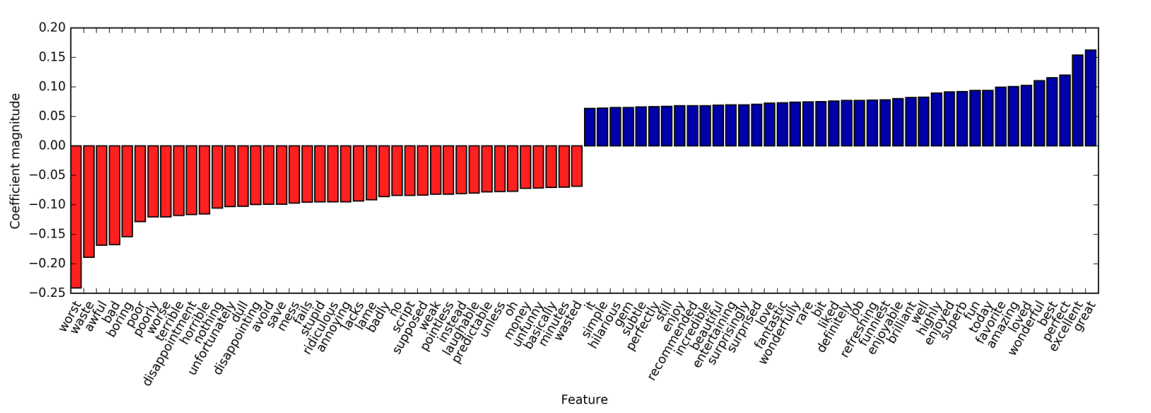
\includegraphics[scale=0.55]{Imagen_Machine/Texto3}
	\caption{Los coeficientes más grandes y más pequeños de las características de regresión logística
		 entrenados en tf-idf}
	\label{Texto3}
\end{figure}



Los coeficientes negativos a la izquierda pertenecen a palabras que según el modelo son indicativas de comentarios negativas, mientras que los coeficientes positivos a la derecha pertenecen a palabras que según el modelo indican comontarios positivos. La mayoría de los términos son bastante intuitivos, como "{}worst"{}, "{}waste"{}, "{}disappointment"{},  y  "{}laughable"{}  ("{}peor"{}, "{}desperdicio"{}, "{}decepción"{} y "{}ridículo"{})  que indica malas críticas de películas, mientras que "{}excellent"{}, "{}wonderful"{}, "{}enjoyable"{},  y 
"{}refreshing"{}  ("{}excelente"{}, "{}maravilloso"{}, "{}agradable"{} y "{}refrescante"{}) indican críticas positivas de películas.
 Algunas palabras son un poco menos claras, como "{}bit"{}, "{}job"{}, y "{}today"{}, pero estas podrían ser parte de frases como "{}good job"{} o "{}best today."{} 
 
\subsection{Bolsa de palabras con más de una palabra \\ (n-Grams)}


% Bag-of-Words with More Than One Word (n-Grams)

Una de las principales desventajas de usar una representación de bolsa de palabras es que el orden de las palabras se descarta por completo. Por lo tanto, las dos cadenas, "{}es malo, no es bueno en absoluto"{}  y  "{}es bueno, no es malo en absoluto"{}  \, tienen exactamente la misma representación, a pesar de que los significados están opuestos.
Poner "{}no"{}  delante de una palabra es sólo un ejemplo  de la  importancia del contexto. 
Afortunadamente, hay una manera de capturar el contexto cuando se utiliza una representación
de bolsa de palabras, no sólo considerando los recuentos de simples tokens, sino también
los recuentos de pares o triples de tokens que aparecen una al lado de la otra.

Los pares de tokens  se conocen como bigrams, los tripletas de tokens se conocen como trigramas, y más generalmente las secuencias de tokens se conocen como n-gramos.
Podemos cambiar el rango de tokens que son  considerados como características cambiando el parámetro {\ttfamily ngram\_range} \, de {\ttfamily CountVectorizer} o  {\ttfamily TfidfVectorizer}. 
El parámetro {\ttfamily  ngram\_range} es una tupla, que consistente en la longitud mínima y máxima de las secuencias de  tokens que son considerados. 

A continuación se expone  un ejemplo  sobre la data Toy  que utilizamos anteriormente:

\begin{lstlisting}%[frame=single]

In[27]:

   print("bards_words:\n{}".format(bards_words))

Out[27]:

   bards_words:
   ['The fool doth think he is wise,',
    'but the wise man knows himself to be a fool']
    
\end{lstlisting}

El valor por defecto  es crear una característica por secuencia de tokens que tenga al menos un token de  longitud  y a lo más un token de longitud, o en otras palabras, exactamente un token de logitud (los tokens individuales también se llaman unigramas):

\begin{lstlisting}%[frame=single]

In[28]:

   cv = CountVectorizer(ngram_range=(1, 1)).fit(bards_words)
   print("Vocabulary size: {}".format(len(cv.vocabulary_)))
   print("Vocabulary:\n{}".format(cv.get_feature_names()))

Out[28]:

   Vocabulary size: 13
   Vocabulary:
   ['be', 'but', 'doth', 'fool', 'he', 'himself', 'is', 'knows', 'man', 'the',
    'think', 'to', 'wise']

\end{lstlisting}

Para ver sólo a los bigrams; es decir, sólo a las secuencias de dos tokens que se suceden 
entre sí, podemos configurar un conjunto {\ttfamily ngram\_range} a (2, 2):

\begin{lstlisting}%[frame=single]

In[29]:

   cv = CountVectorizer(ngram_range=(2, 2)).fit(bards_words)
   print("Vocabulary size: {}".format(len(cv.vocabulary_)))
   print("Vocabulary:\n{}".format(cv.get_feature_names()))

Out[29]:
  
   Vocabulary size: 14
   Vocabulary:
   ['be fool', 'but the', 'doth think', 'fool doth', 'he is', 'himself to',
    'is wise', 'knows himself', 'man knows', 'the fool', 'the wise',
    'think he', 'to be', 'wise man']

\end{lstlisting}


El uso de secuencias más largas de tokens generalmente resulta en muchas más características,
y en características más específicas. No hay un bigram común entre las dos frases en
 {\ttfamily bard\_words}:


\begin{lstlisting}%[frame=single]

In[30]:

   print("Transformed data (dense):\n{}".format(
          cv.transform(bards_words).toarray()))

Out[30]:

   Transformed data (dense):
   [[0 0 1 1 1 0 1 0 0 1 0 1 0 0]
    [1 1 0 0 0 1 0 1 1 0 1 0 1 1]]

\end{lstlisting}

Para la mayoría de las aplicaciones, el número mínimo de tokens debe ser uno, 
como  palabras  únicas que con frecuencia capturan gran significado. Agregar un bigrams en 
la mayoría de los casos ayuda. 

Agregando secuencias más largas, hasta  5-grams, también pueden ayudar, pero esto conducirá 
a una explosión de la cantidad de características y podría conducir a un sobreajuste, 
ya que habrá muchas características específicas. 

En principio, el número de bigrams podría ser el número de unigrams al cuadrado y el número de trigrams podría ser el número de unigrams a la potencia de tres, lo que lleva a espacios de características muy grandes. En la práctica, el número alto de los n-grams  que realmente aparecen en los datos son mucho más pequeños, debido a la estructura  del idioma (inglés), aunque todavía es grande.

A continuación se muestra   como se ve el uso de unigrams, bigrams y trigrams sobre {\ttfamily bards\_words}:

\begin{lstlisting}%[frame=single]

In[31]:

   cv = CountVectorizer(ngram_range=(1, 3)).fit(bards_words)
   print("Vocabulary size: {}".format(len(cv.vocabulary_)))
   print("Vocabulary:\n{}".format(cv.get_feature_names()))

Out[31]:

   Vocabulary size: 39
   Vocabulary:
   ['be', 'be fool', 'but', 'but the', 'but the wise', 'doth', 'doth think',
    'doth think he', 'fool', 'fool doth', 'fool doth think', 'he', 'he is',
    'he is wise', 'himself', 'himself to', 'himself to be', 'is', 'is wise',
    'knows', 'knows himself', 'knows himself to', 'man', 'man knows',
    'man knows himself', 'the', 'the fool', 'the fool doth', 'the wise',
    'the wise man', 'think', 'think he', 'think he is', 'to', 'to be',
    'to be fool', 'wise', 'wise man', 'wise man knows']

\end{lstlisting}

Vamos a probar el {\ttfamily TfidfVectorizer} en los datos de comentarios de películas IMDb 
y encontrar la mejor configuración del rango  n-gram   utilizando una búsqueda de cuadrícula: 

\begin{lstlisting}%[frame=single]

In[32]:

   pipe = make_pipeline(TfidfVectorizer(min_df=5), LogisticRegression())
   # running the grid search takes a long time because of the
   # relatively large grid and the inclusion of trigrams
   param_grid = {"logisticregression__C": [0.001, 0.01, 0.1, 1, 10, 100],
                 "tfidfvectorizer__ngram_range": [(1, 1), (1, 2), (1, 3)]}
  
   grid = GridSearchCV(pipe, param_grid, cv=5)
   grid.fit(text_train, y_train)
   print("Best cross-validation score: {:.2f}".format(grid.best_score_))
   print("Best parameters:\n{}".format(grid.best_params_))

Out[32]:

   Best cross-validation score: 0.91
   Best parameters:
   {'tfidfvectorizer__ngram_range': (1, 3), 'logisticregression__C': 100}

\end{lstlisting}

Como se puede ver en los resultados, hemos mejorado el rendimiento un poco más que un 
por ciento mediante la adición características de  bigram  y  de trigrama. 
Podemos visualizar la exactitud (accuracy) de validación cruzada como una función 
del parámetro {\ttfamily ngram\_range} y C como un mapa caliente,   como se hizo en 
el capítulo \ref{Cap5} (ver Figura \ref{Texto4}):

\begin{lstlisting}%[frame=single]

In[33]:

   # extract scores from grid_search
   scores = grid.cv_results_['mean_test_score'].reshape(-1, 3).T
   # visualize heat map
   heatmap = mglearn.tools.heatmap(
       scores, xlabel="C", ylabel="ngram_range", cmap="viridis", fmt="%.3f",
       xticklabels=param_grid['logisticregression__C'],
       yticklabels=param_grid['tfidfvectorizer__ngram_range'])
   plt.colorbar(heatmap)

\end{lstlisting}

\begin{figure}[h!]
	\centering
	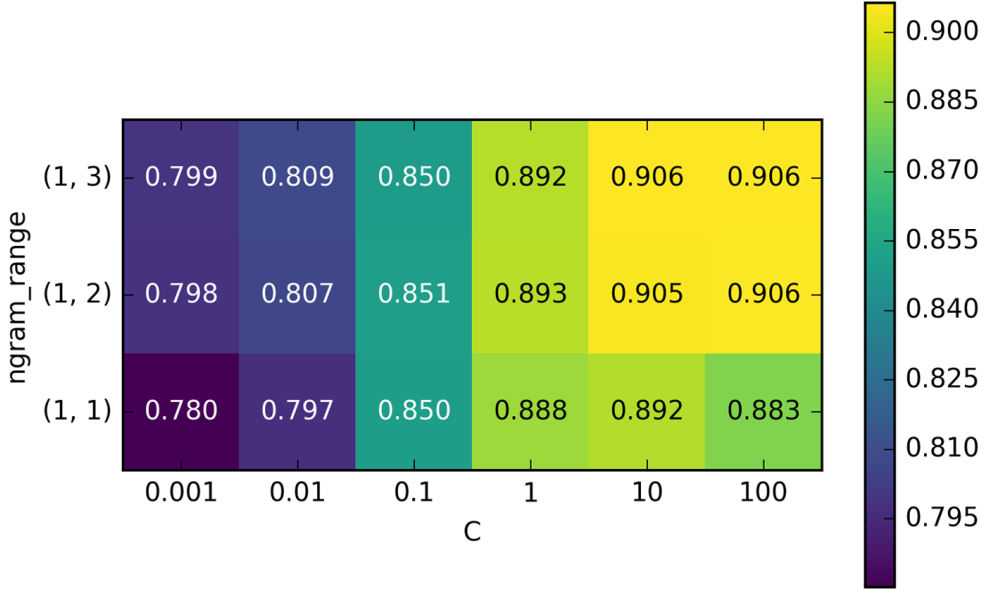
\includegraphics[scale=0.55]{Imagen_Machine/Texto4}
	\caption{Visualización del mapa caliente de la exactitud media de la validación cruzada como una función de los parámetros {\ttfamily ngram\_range} y C}
	\label{Texto4}
\end{figure}

En el  mapa caliente podemos ver que el uso de bigrams aumenta el rendimiento un poco, mientras que la adición de trigramas sólo proporciona un beneficio muy pequeño en términos de exactitud. Para entender mejor cómo mejoró el modelo, podemos visualizar la importancia de los coeficiente  para el mejor modelo, que incluye unigrams, bigrams y trigrams (ver Figura \ref{Texto5}):

\begin{lstlisting}%[frame=single]

In[34]:

   # extract feature names and coefficients
   vect = grid.best_estimator_.named_steps['tfidfvectorizer']
   feature_names = np.array(vect.get_feature_names())
   coef = grid.best_estimator_.named_steps['logisticregression'].coef_
   mglearn.tools.visualize_coefficients(coef, feature_names,
                                        n_top_features=40)

\end{lstlisting}

\begin{figure}[h!]
	\centering
	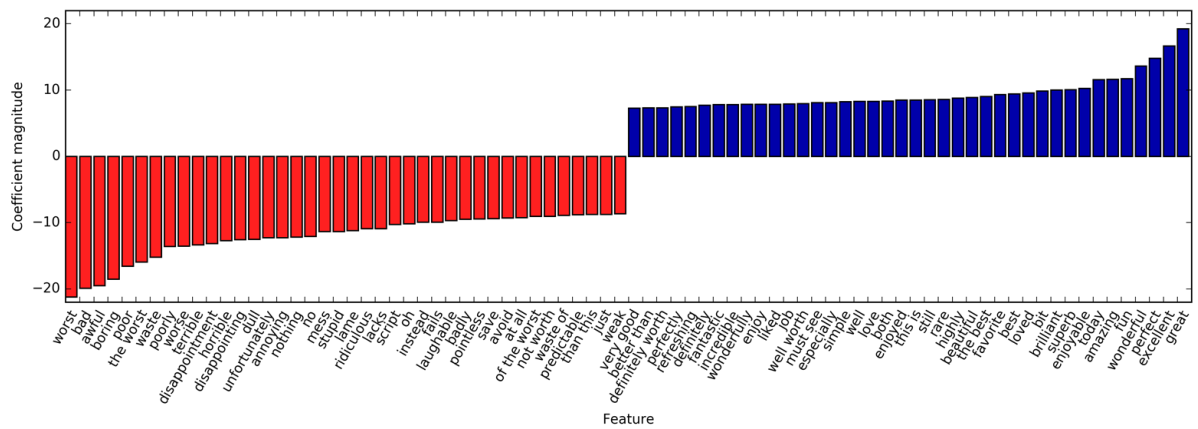
\includegraphics[scale=0.55]{Imagen_Machine/Texto5}
	\caption{Características más importantes al usar unigrams, bigrams y trigrams 
		con el reescalado  tf-idf}
	\label{Texto5}
\end{figure}

Hay características particularmente interesantes que contienen la palabra "{}worth"{} (valor)
que no estaban presentes en el modelo unigram: "{}not worth"{}  es indicativo de una comentario negativa, mientras que "{}definitely worth"{}  y "{}well worth"{}  son indicativos de una revisión positiva. 
Este es un primer ejemplo de contexto que influye en el significado de la palabra "{}worth"{}.


A continuación, visualizaremos sólo trigramas, para proporcionar una mayor comprensión de por qué estas características son útiles. Muchos de los bigrams y trigrams útiles consisten en palabras comunes que no serían informativos por sí solos, como en las frases "{}none of the"{},  "{}the only good"{}, "{}on and on"{}, "{}this is one"{}, "{}of the most"{} ("{}ninguno de los"{},  "{}el único bueno"{}, "{}incesantemente"{}, "{}esto es uno"{}, "{}de la mayoría"{}),  y así sucesivamente. 
Sin embargo, el impacto de estas características es bastante limitado en comparación con la importancia de las características de unigram, como se puede ver en la Figura \ref{Texto5}:

\begin{lstlisting}%[frame=single]

In[35]:

   # find 3-gram features
   mask = np.array(
           [len(feature.split(" "))  for feature in feature_names]) == 3
   # visualize only 3-gram features
   mglearn.tools.visualize_coefficients(
           coef.ravel()[mask],  feature_names[mask], n_top_features=40)

\end{lstlisting}

\begin{figure}[h!]
	\centering
	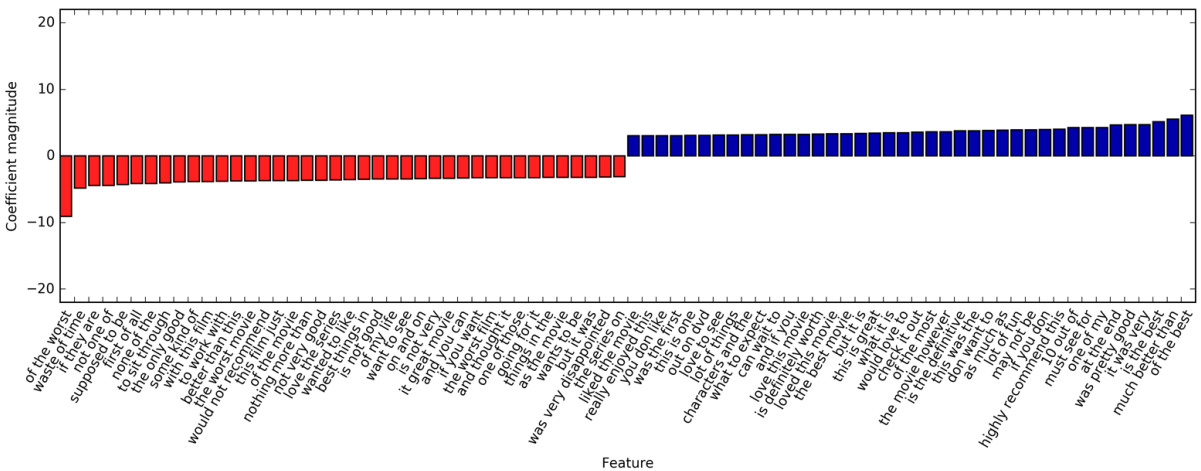
\includegraphics[scale=0.55]{Imagen_Machine/Texto7}
	\caption{Visualización  sólo de las características más importantes  del modelo trigram}
	\label{Texto7}
\end{figure}

\newpage
% siendo cada n-grama una secuencia de n palabras consecutivas
%  documentos del corpus (idf).
%  https://en.wikipedia.org/wiki/Lexical_analysis#Tokenization
%  https://towardsdatascience.com/why-you-should-avoid-removing-stopwords-aa7a353d2a52

\subsection{Tokenización avanzada,  Stemming y lematización}
%Como se mencionó anteriormente,

La extracción de características en {\ttfamily  CountVectorizer}  y  {\ttfamily TfidfVectorizer}  es relativamente simple, y   muchos métodos  más elaborados son posibles.
 Un paso particular que a menudo   mejora   las  aplicaciones de procesamiento de texto más sofisticadas,
es el primer paso en el modelo de bolsa de palabras: tokenización. Este paso define lo que
constituye una palabra para la extracción de características.\\


Vimos anteriormente que el vocabulario a menudo contiene versiones singulares y plurales de
algunas palabras, como en "{}inconveniente"{} y "{}inconvenientes"{}, "{}cajón"{} y "{}cajones"{}, y
"{}dibujo"{} y "{}dibujos"{}.   A los efectos de un modelo de bolsa de palabras, la semántica
de "{}inconveniente"{ }  y  "{}inconvenientes"{ } están tan cerca que distinguirlos sólo
aumentar el sobreajuste y no permiten que el modelo explote por completo 
los datos de entrenamiento.


Similarmente, encontramos que el vocabulario incluye palabras como "{}reemplazar"{},
 "{}reemplazado"{}, "{}reemplazadamente"{},  "{}reemplazos"{}  y  "{}reemplazando"{}, 
 que son formas verbales diferentes y un sustantivo relacionado con el verbo "{}reemplazar"{}.  
 De manera similar al tener formas singulares y plurales de un sustantivo, tratando  diferentes formas verbales y palabras relacionadas como símbolos distintos es desventajoso  para construir un modelo que generalice bien.\\

  
Este problema se puede superar representando cada palabra usando la raíz de la 
palabra\footnote{ \scriptsize{Raíz de una palabra: La parte común de las palabras se llama raíz, también 
	conocido como lexema. La raíz de una palabra es la parte de la palabra que no cambia. 
	A partir de una raíz podemos formar palabras que son relacionadas por su significado}} (word stem)
que involucra identificar (o combinar) todas las palabras que tienen la misma raíz.
 Si esto se realiza mediante el uso de una heurística basada en reglas, como descartar 
 sufijos comunes, generalmente es referido como stemming  (derivación).  Si, en cambio, se utiliza 
 un diccionario  de formas de palabras conocidas (un sistema explícito y verificado 
 por humanos), y  se toma  en cuenta el papel de la palabra en la oración, 
 el proceso se denomina lematización y la forma estandarizada de la palabra se 
 conoce como lema.  
Ambos métodos de procesamiento, lematización y stemming, son formas de normalización
  que intentan extraer alguna forma normal de una palabra.   Otro caso interesante de normalización es la corrección ortográfica, que puede ser
útil en la práctica pero está fuera del alcance de este libro.\\

Para obtener una mejor comprensión de la normalización, comparemos un método para stemming,
el método stemmer  Porter{\footnote{\scriptsize	{ algoritmo de Porter es un algoritmo que asegura que
 la forma de las palabras no penalice la frecuencia de éstas. Es decir, una palabra puede
  estar conjugada en cualquier género, número, persona, y solo se considerará como un solo término.}}}, 
una colección ampliamente utilizada de heurísticas (aquí importada del paquete {\ttfamily  nltk}) 
 para lemmatización como se implementa en el paquete {\ttfamily spacy}\footnote{ \scriptsize{ más detalles
 sobre la interfaz, consulte la documentación \href{http://www.nltk.org/}{\textcolor{vino}{\ttfamily nltk} }} y \href{https://spacy.io/}{\textcolor{vino}{\ttfamily spacy} }. Aquí sólo nos interesamos en los principios generales.}:


\begin{lstlisting}%[frame=single]

In[36]:

   import spacy
   import nltk
   
   # load spacy's English-language models
   en_nlp = spacy.load('en')
   # instantiate nltk's Porter stemmer
   stemmer = nltk.stem.PorterStemmer()
   
   # define function to compare lemmatization in spacy with stemming in nltk
   def compare_normalization(doc):
       # tokenize document in spacy
       doc_spacy = en_nlp(doc)
       # print lemmas found by spacy
       print("Lemmatization:")
       print([token.lemma_ for token in doc_spacy])
       # print tokens found by Porter stemmer
       print("Stemming:")
       print([stemmer.stem(token.norm_.lower()) for token in doc_spacy])

\end{lstlisting}

Vamos a comparar lemmatización y el stemmer Porter en una frase diseñada para mostrar algunas de las diferencias:

\begin{lstlisting}%[frame=single]

In[37]:

   compare_normalization(u"Our meeting today was worse than yesterday, "
   "I'm scared of meeting the clients tomorrow.")

Out[37]:

   Lemmatization:
   ['our', 'meeting', 'today', 'be', 'bad', 'than', 'yesterday', ',', 'i',
    'be', 'scared', 'of', 'meet', 'the', 'client', 'tomorrow', '.']
   Stemming:
   ['our', 'meet', 'today', 'wa', 'wors', 'than', 'yesterday', ',', 'i', 
    'm', 'scare', 'of', 'meet', 'the', 'client', 'tomorrow', '.']

\end{lstlisting}

Stemming está siempre  restringido  a recortar la palabra a una stem (raíz), así que "{}was"{} 
se convierte en "{}wa"{}, mientras que la lemmatización puede recuperar la forma de
 base del verbo  correcta, "{}be"{}. De manera similar, la lemmatización puede normalizar  
 "{}worse"{}  a "{}bad"{}  ( "{}peor"{} a "{}malo"{}), mientras que stemming 
  produce  "{}wors"{}. 
Otra diferencia importante es que stemming  reduce ambos casos  "{}meeting"{ } a
"{}meet"{ }   ("{}reunión"{}  a "{}reunirse"{}).
 Usando lematización, la primera ocurrencia  de  "{}meeting"{}   ("{}reunión"{})  se reconoce
  como un sustantivo y se deja como está, mientras que la segunda ocurrencia se reconoce como un 
 verbo y se reduce a  "{}meet"{} ("{}reunión"{}).  \\


En general, la lemmatización es un proceso mucho más complicado que el stemming, 
pero generalmente produce mejores resultados  que el stemming cuando se utiliza 
para  normalización  los tokens de aprendizaje automático.\\


Mientras que {\ttfamily scikit-learn} no implementa ninguna forma de normalización, {\ttfamily CountVectorizer} permite especificar su propio tokenizador  para convertir cada documento 
en una lista de tokens usando el parámetro {\ttfamily tokenizer}. 
Podemos usar la lematización de {\ttfamily spacy} para crear un invocable que tomará una 
cadena y producirá una lista de lemas:




\begin{lstlisting}%[frame=single]

In[38]:

   # Technicality: we want to use the regexp-based tokenizer
   # that is used by CountVectorizer and only use the lemmatization
   # from spacy. To this end, we replace en_nlp.tokenizer 
   # (the spacy tokenizer) with the regexp-based tokenization.
   import re
   # regexp used in CountVectorizer
   regexp = re.compile('(?u)\\b\\w\\w+\\b')
   
   # load spacy language model and save old tokenizer
   en_nlp = spacy.load('en')
   old_tokenizer = en_nlp.tokenizer
   # replace the tokenizer with the preceding regexp
   en_nlp.tokenizer = lambda string: old_tokenizer.tokens_from_list(
       regexp.findall(string))
   
   # create a custom tokenizer using the spacy document processing
   #  pipeline
   # (now using our own tokenizer)
   def custom_tokenizer(document):
       doc_spacy = en_nlp(document, entity=False, parse=False)
       return [token.lemma_ for token in doc_spacy]
       
   # define a count vectorizer with the custom tokenizer
   lemma_vect = CountVectorizer(tokenizer=custom_tokenizer, min_df=5)

\end{lstlisting}

Transformemos los datos e inspeccionemos el tamaño del vocabulario:

\begin{lstlisting}%[frame=single]

In[39]:

   # transform text_train using CountVectorizer with lemmatization
   X_train_lemma = lemma_vect.fit_transform(text_train)
   print("X_train_lemma.shape: {}".format(X_train_lemma.shape))
   
   # standard CountVectorizer for reference
   vect = CountVectorizer(min_df=5).fit(text_train)
   X_train = vect.transform(text_train)
   print("X_train.shape: {}".format(X_train.shape))

Out[39]:

   X_train_lemma.shape: (25000, 21596)
   X_train.shape: (25000, 27271)

\end{lstlisting}

\noindent Como se puede ver en la salida, el método lemmatización redujo el número de 
características de 27.271 (con el procesamiento {\ttfamily CountVectorizer estándar}) 
a 21.596. La lemmatización puede ser vista como una tipo de regularización, ya que combina
 ciertas características.
 Por lo tanto, esperamos que la lemmatización mejore el rendimiento más cuando la data es pequeña.
 Para ilustrar cómo la lemmatización puede ayudar, usaremos {\ttfamily StratifiedShuffleSplit} para la validación cruzada, usando solo el 1\% de los datos para conjunto de entrenamiento y el resto como datos de prueba:

\begin{lstlisting}%[frame=single]

In[40]:

   # build a grid search using only 1% of the data as the training set
   from sklearn.model_selection import StratifiedShuffleSplit
   
   param_grid = {'C': [0.001, 0.01, 0.1, 1, 10]}
   cv = StratifiedShuffleSplit(n_iter=5, test_size=0.99,
                               train_size=0.01, random_state=0)
   grid = GridSearchCV(LogisticRegression(), param_grid, cv=cv)
   # perform grid search with standard CountVectorizer
   grid.fit(X_train, y_train)
   print("Best cross-validation score "
         "(standard CountVectorizer): {:.3f}".format(grid.best_score_))
   # perform grid search with lemmatization
   grid.fit(X_train_lemma, y_train)
   print("Best cross-validation score "
         "(lemmatization): {:.3f}".format(grid.best_score_))

Out[40]:

   Best cross-validation score (standard CountVectorizer): 0.721
   Best cross-validation score (lemmatization): 0.731

\end{lstlisting}

En este caso, la lemmatización proporcionó una modesta mejora en el desempeño.
 Al igual que con muchas de las diferentes técnicas de extracción de características,
 el resultado varía dependiendo de la dataset. 
 
 La lemmatización y el stemming a veces  pueden ayudar a construir modelos mejores (o al menos más compactos), por lo que le   sugerimos que pruebe estas técnicas  tratando de exprimir la última gota 
  de rendimiento en una tarea en particular.

\subsection{Modelado de temas y Clúster de documentos}

Una técnica particular que a menudo se aplica a los datos de texto es el
 modelado de temas o tópicos, que es un término general  que describe la tarea de 
 asignar cada documento a uno o varios temas, por lo general sin supervisión. 
 Un buen ejemplo de este caso  son los datos noticiosos, que podrían clasificarse en
 temas como "política", "deportes", "finanzas", etc. Si a cada documento se le 
 asigna un sólo tema, esta es la tarea de agrupar los documentos, como se discute
 en el Capítulo \ref{Cap3}. 
Si cada documento puede tener más de un tema,  
la tarea se relaciona con los métodos de descomposición del Capítulo \ref{Cap3}.  Cada uno de los componentes  aprendidos  corresponde a un tema, y los coeficientes de los componentes en la representación de un documento nos dicen lo fuerte que es  la  relación del documento con un tema en particular. A menudo, cuando la gente habla de modelado de temas, se refieren a un método de descomposición parcial llamado \emph{Asignación de Dirichlet latente} (Latent Dirichlet Allocation, LDA)\footnote{Hay otro modelo de aprendizaje automático que también se abrevia a como LDA: Linear Discriminant Analysis, un modelo de clasificación lineal. Esto lleva a bastante confusión. En este libro, LDA se refiere a la Asignación Dirichlet Latente.}.


\subsection{Asignación de Latente  Dirichlet  LDA} 
%Latent Dirichlet Allocation

Intuitivamente, el modelo LDA intenta encontrar grupos de palabras (los temas) que aparecen frecuentemente juntos. LDA también requiere que cada documento pueda ser entendido como una "{}mezcla"{}  de un subconjunto de los temas. Es importante entender que para el modelo de aprendizaje automático un "{}tema"{} podría no ser lo que normalmente llamaríamos un tema en el discurso diario, pero que se asemeja más a los componentes extraídos por  PCA  o  NMF (que discutimos en el capítulo \ref{Cap3}), que puede o no tener un significado semántico.

Incluso si hay un significado semántico para un "{}tema"{ }  de  LDA, puede que no sea algo que normalmente llamamos un tema.   Volviendo al ejemplo de los artículos de noticias, podríamos
tener  una colección de artículos sobre deportes, política y finanzas, escritos por dos
autores. En un artículo sobre política, podríamos esperar ver palabras como "{}gobernador"{}, "{}votar"{}
"{}Fiesta"{}, etc., mientras que en otro artículo de deportes podemos esperar palabras como "{}equipo"{}, "{}puntuación"{}  y  "{}temporada."{} 
Sin embargo, estos no son los únicos grupos de palabras que podríamos esperar que aparezcan juntas.
Los dos reporteros podría preferir diferentes frases o diferentes opciones de palabras. 
 Quizás a uno de ellos le guste utilizar la palabra "{}demarcar"{} y a el otro le gusta la palabra "{}polarizar"{}.  Otros "{}temas"{} serían "{}palabras de uso frecuente por el reportero A"{}  y  "{}palabras de uso frecuente por el reportero B"{},  aunque estos no son temas en el sentido habitual de la palabra. \\


Vamos a aplicar LDA a la data reseñas de peliculas (review  movie) para ver cómo 
funciona en la práctica. Para los modelos de documentos de texto sin supervisión, a menudo es bueno eliminar palabras muy comunes, ya que de lo contrario podrían dominar el análisis. Eliminaremos las palabras que aparecen  al menos en un 15 por ciento de los documentos, y limitaremos el modelo de bolsa de palabras (bag-of-words) a las 10.000 palabras que son más comunes después de eliminar un  máximo de  15 por ciento: 

\begin{lstlisting}%[frame=single]

In[41]:

   vect = CountVectorizer(max_features=10000, max_df=.15)
   X = vect.fit_transform(text_train)
   
\end{lstlisting}

Vamos a entrenar el aprendizaje  de  un modelo  con 10 tópicos (temas), que son pocos y suficiente
 como para que podamos verlos  a todos. De manera similar a los componentes en  NMF, 
los temas no tienen un orden inherente, y cambiar el número de temas cambiará todos los temas\footnote{De hecho, NMF y LDA resuelven problemas muy relacionados, y también podríamos utilizar NMF para extraer temas}.  Usaremos el método de aprendizaje "{}por lotes"{} ("{}batch"{}),  que es algo más lento 
que el predeterminado  ("{}online"{}),  pero por lo general proporciona mejores resultados, y aumentar  el \:  "{}{\ttfamily max\_iter}"{}    también puede conducir a mejores modelos:

\begin{lstlisting}%[frame=single]

In[42]:

   from sklearn.decomposition import LatentDirichletAllocation
   lda = LatentDirichletAllocation(n_topics=10, learning_method="batch",
                                   max_iter=25, random_state=0)
   # We build the model and transform the data in one step
   # Computing transform takes some time,
   # and we can save time by doing both at once
   document_topics = lda.fit_transform(X)
   
\end{lstlisting}

Al igual que los métodos de descomposición que vimos en el capítulo \ref{Cap3}, {\ttfamily LatentDirichletAllocation}  tiene un atributo {\ttfamily components\_} que almacena la
 importancia de cada palabra para cada tema. El tamaño de  {\ttfamily components\_} \: es  
 {\ttfamily (n\_topics, n\_words)}:

\begin{lstlisting}%[frame=single]

In[43]:
   
   lda.components_.shape

Out[43]:
   
   (10, 10000)

\end{lstlisting}

Para entender mejor lo que significan los diferentes temas, veremos las palabras más 
importantes para cada uno de los temas. La función {\ttfamily print\_topics}  proporciona un 
formato agradable para estas características:


%%%%%%%%%%%%%%%%%%%%%%%%%%%%%%%%%%%%%%%%%%%%%%%%%%%%%%%%%%%%%%%
%%  Aqui va In[44]
%%%%%%%%%%%%%%%%%%%%%%%%%%%%%%%%%%%%%%%%%%%%%%%%%%%%%%%%%%%%%%%


\begin{lstlisting}%[frame=single]

In[44]:

   # For each topic (a row in the components_), sort the features (ascending)
   # Invert rows with [:, ::-1] to make sorting descending
   sorting = np.argsort(lda.components_, axis=1)[:, ::-1]
   # Get the feature names from the vectorizer
   feature_names = np.array(vect.get_feature_names())

In[45]:

   # Print out the 10 topics:
   mglearn.tools.print_topics(topics=range(10), feature_names=feature_names,
                              sorting=sorting, topics_per_chunk=5, n_words=10)

Out[45]
\end{lstlisting}
\vspace{-0.45cm}
\begin{figure}[h!]
	%	\centering
	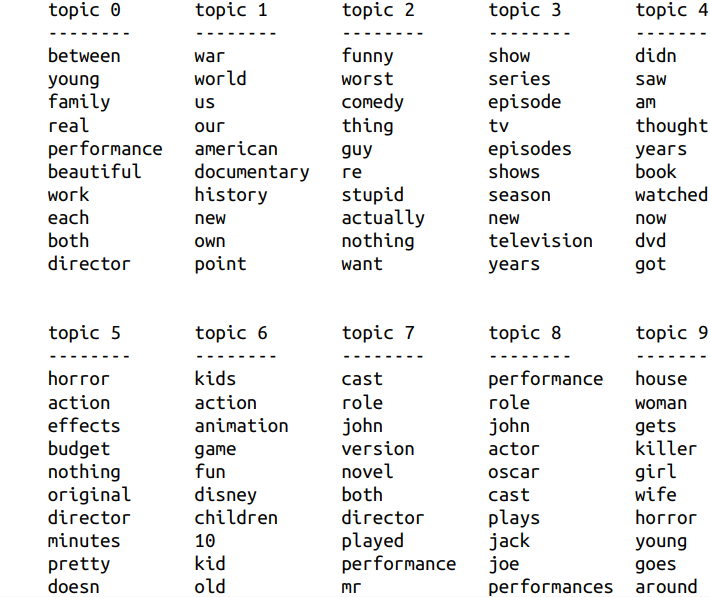
\includegraphics[scale=0.65]{Imagen_Machine/Out44}
	%\caption{Matriz de confusión para clasificación binaria}
	%	\label{Out44}
\end{figure}

\newpage 
Juzgando por las palabras importantes, el tema 1 parece ser sobre películas históricas y de guerra (bélicos), el tema 2 podría ser sobre malas comedias, el tema 3 podría ser sobre series de televisión. El tema 4 parece capturar algunas palabras muy comunes, mientras que el tema 6 parece ser sobre sobre películas infantiles  y el tema 8 parece capturar críticas relacionadas con premios. Utilizando sólo 10 temas, cada uno de los temas tiene que ser muy amplio, para que juntos puedan cubrir todos los diferentes tipos de comentarios  en la dataset.\\


A continuación, se entrena otro modelo de aprendizaje, esta vez con 100 temas. El uso de más temas hace el análisis mucho más difícil, pero hace más probable que los temas puedan   especializarse en subconjuntos interesantes de la data:

%%%%%%%%%%%%%%%%%%%%%%%%%%%%%%%%%%%%%%%%%%%%%%%%%%%%%%%%%%%%%%%
%%  Aqui no  va In[44]
%%%%%%%%%%%%%%%%%%%%%%%%%%%%%%%%%%%%%%%%%%%%%%%%%%%%%%%%%%%%%%%

\begin{lstlisting}%[frame=single]


In[46]:

   lda100 = LatentDirichletAllocation(n_topics=100, learning_method="batch",
                                      max_iter=25, random_state=0)
   document_topics100 = lda100.fit_transform(X)


\end{lstlisting}

\noindent   Observando todos los 100 temas sería un poco abrumador, así que seleccionamos algunos temas de interés y representativos:

\begin{lstlisting}%[frame=single]


In[47]:

   topics = np.array([7, 16, 24, 25, 28, 36, 37, 45, 51, 53, 54, 63, 89, 97])
   
   sorting = np.argsort(lda100.components_, axis=1)[:, ::-1]
   feature_names = np.array(vect.get_feature_names())
   mglearn.tools.print_topics(topics=topics, feature_names=feature_names,
                              sorting=sorting, topics_per_chunk=7, n_words=20)

Out[47]:

\end{lstlisting}    %   error Out[48]
\vspace{-0.65cm}
\begin{figure}[h!]
	%	\centering
	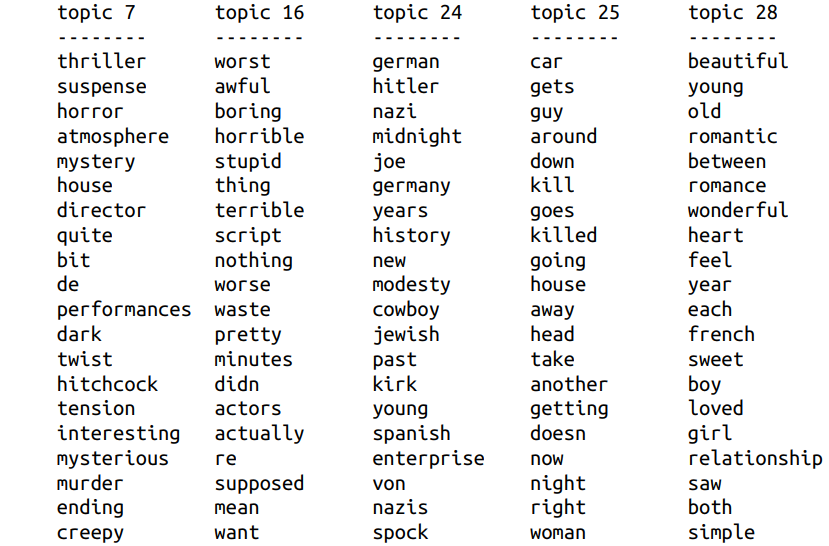
\includegraphics[scale=0.55]{Imagen_Machine/Out48}
	%\caption{Matriz de confusión para clasificación binaria}
	%	\label{Out48}
\end{figure}

\vspace{-3.5cm}
\begin{figure}[h!]
	%	\centering
	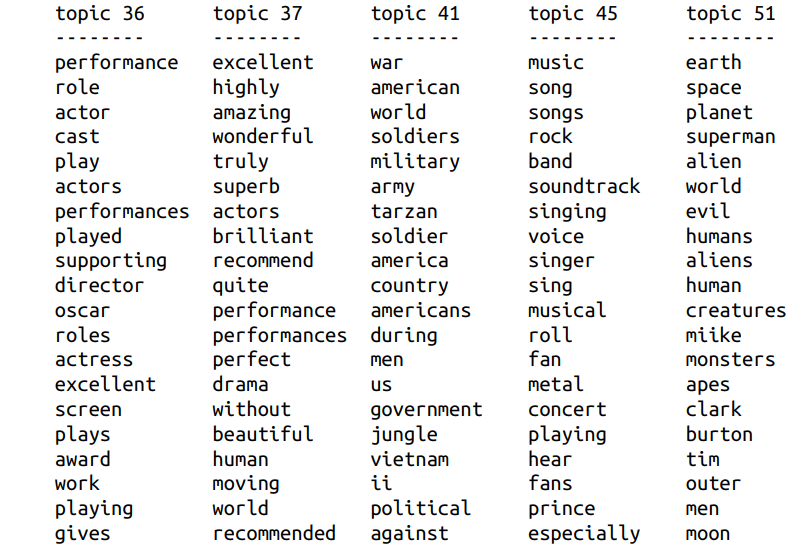
\includegraphics[scale=0.55]{Imagen_Machine/Out48a}
	%\caption{Matriz de confusión para clasificación binaria}
	%	\label{Out48b}
\end{figure}
\vspace{-0.5cm}\hspace{-0.9cm}
\begin{minipage}[t]{1\textwidth}
	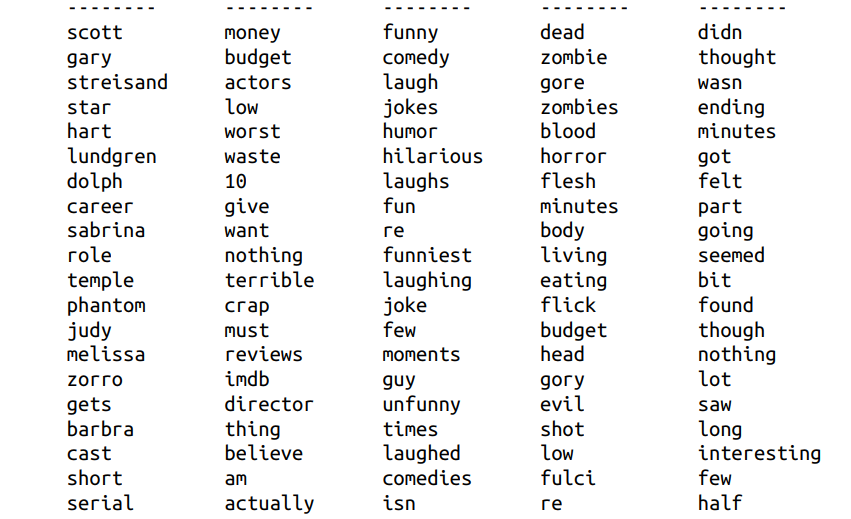
\includegraphics[scale=0.55]{Imagen_Machine/Out48b}
\end{minipage}


Los temas que hemos extraído esta vez parecen ser más específicos, aunque muchos son difíciles de interpretar. El tema 7 parece versar sobre películas de terror y suspenso (thrillers); los temas 16 y 54 parecen captar malas críticas, mientras que el tema 63 en su mayoría parece captar críticas positivas de comedias. Si queremos hacer más inferencias usando los temas que fueron descubiertos, debemos confirmar la intuición que ganamos al ver las palabras de mayor rango  para cada tema observando los documentos que se asignan a estos temas. Por ejemplo, al tema 45 parece versar sobre la música. Vamos a comprobar qué tipos de reseñas se asignan a este tema:


\begin{lstlisting}

In[49]:
   
   # sort by weight of "music" topic 45
   music = np.argsort(document_topics100[:, 45])[::-1]
   # print the five documents where the topic is most important
   for i in music[:10]:
   # pshow first two sentences
   print(b".".join(text_train[i].split(b".")[:2]) + b".\n")

Out[49]:

   b'I love this movie and never get tired of watching. The music in it is 
     great.\n'
   b"I enjoyed Still Crazy more than any film I have seen in years. A 
     successful band from the 70's decide to give it another try.\n"
   b'Hollywood Hotel was the last movie musical that Busby Berkeley 
     directed  for Warner Bros. His directing style had changed or
     evolved to the point that this film does not contain his 
     signature overhead shots or huge production numbers with thousands 
     of extras.\n'
   b"What happens to washed up rock-n-roll stars in the late 1990's?
     They launch a comeback / reunion tour. At least, that's what the
     members of Strange Fruit, a (fictional) 70's stadium rock group do.\n"
   b'As a big-time Prince fan of the last three to four years, I really 
     can\'t believe I\'ve only just got round to watching "Purple Rain". 
     The brand  new  2-disc anniversary Special Edition led me to buy it.\n'
   b"This film is worth seeing alone for Jared Harris' outstanding portrayal
     of John Lennon. It doesn't matter that Harris doesn't exactly resemble
     Lennon; his mannerisms, expressions, posture, accent and attitude are
     pure Lennon.\n"
   b"The funky, yet strictly second-tier British glam-rock band Strange 
     Fruit breaks up at the end of the wild'n'wacky excess-ridden 70's. The 
     individual band members go their separate ways and uncomfortably settle
     into lackluster middle age in the dull and uneventful 90's: morose 
     keyboardist Stephen Rea winds up penniless and down on his luck, vain, 
     neurotic, pretentious lead singer Bill Nighy tries (and fails) to
     pursue a floundering solo career, paranoid drummer Timothy Spall 
     resides in obscurity on a remote farm so he can avoid paying a hefty 
     back taxes debt, and surly bass player Jimmy Nail installs roofs for 
     a living.\n"
   b"I just finished reading a book on Anita Loos' work and the photo in TCM
     Magazine of MacDonald in her angel costume looked great 
     (impressive wings), so I thought I'd watch this movie. I'd never heard 
     of the film before, so I had no preconceived notions about it 
     whatsoever.\n"
   b'I love this movie!!! Purple Rain came out the year I was born and it
     has had my heart since I can remember. Prince is so tight in this 
     movie.\n'
   b"This movie is sort of a Carrie meets Heavy Metal. It's about a 
     highschool guy who gets picked on alot and he totally gets revenge with
     the help of a Heavy Metal ghost.\n"

\end{lstlisting}


Como podemos ver, este tema cubre una amplia variedad  de comentarios centrados en música, desde comedias musicales, a películas biográficas, para  algún  género difícil de especificar   en el último comentario.   Otra forma interesante para inspeccionar los tópicos,   es ver cuánto peso se le da a cada tema,   sumando  todos tópicos  {\ttfamily  document\_topics}  de todas las  reseñas.  Nombramos cada tema por las dos palabras más comunes. En la  figura \ref{LDA8} se muestran las ponderaciones tópicos  aprendidos:


\begin{lstlisting}%[frame=single]

In[50]:

   fig, ax = plt.subplots(1, 2, figsize=(10, 10))
   topic_names = ["{:>2} ".format(i) + " ".join(words)
                 for i, words in enumerate(feature_names[sorting[:, :2]])]
   # two column bar chart:
   for col in [0, 1]:
       start = col * 50
       end = (col + 1) * 50
       ax[col].barh(np.arange(50), 
                    np.sum(document_topics100, axis=0)[start:end])
       ax[col].set_yticks(np.arange(50))
       ax[col].set_yticklabels(topic_names[start:end], ha="left", va="top")
       ax[col].invert_yaxis()
       ax[col].set_xlim(0, 2000)
       yax = ax[col].get_yaxis()
       yax.set_tick_params(pad=130)
   plt.tight_layout()

\end{lstlisting}

\begin{figure}[h!]
	\centering
	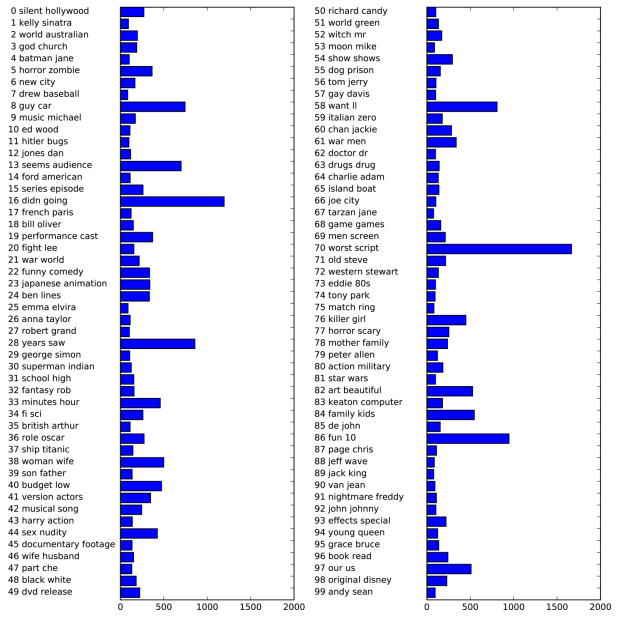
\includegraphics[width=1.03\textwidth]{Imagen_Machine/Texto8}
	\caption{Pesos temáticos aprendidos por LDA}
\label{LDA8}
\end{figure}


De acuerdo con el gráfico de la figura \ref{LDA8}, los temas más importantes son 97, que parece consistir principalmente en stopwords (palabras vacías), posiblemente  con una ligera dirección negativa; el tema 16,  claramente trata sobre malas críticas;
seguido de algunos temas específicos de género, el  36 y 37, ambos parecen contener palabras elogiosas.\\

Parece que LDA descubrió principalmente dos tipos de temas,  género específico y específica valoración
 (genre-specific y ratingspecific), además de varios temas   poco  específicos.   Este es un descubrimiento interesante, ya que la mayoría de las reseñas están hechas  por algunos comentarios específicos de películas y algunos  que justifican o enfatizan la valoración (rating).
   
Los modelos de temas como LDA son métodos interesantes para comprender grandes corpus de texto en
la ausencia de etiquetas,  o  como aquí, incluso si hay etiquetas disponibles. 
El algoritmo LDA es aleatorizado, sin embargo,  cambiar el parámetro 
 {\ttfamily random\_state} puede conducir resultados muy diferentes.


 Si bien identificar temas puede ser útil, cualquier conclusión que saques de un modelo no supervisado debe tomarse con un grano de sal, y recomendamos verificar tu intuición observando los documentos en un tema específico. 
 Los temas producidos por el método {\ttfamily LDA.transform}  también pueden utilizarse a veces como una representación conjunta para el aprendizaje supervisado. Esto es particularmente útil cuando se dispone de pocos ejemplos para entrenar.



\section{Resumen y perspectivas}


En este capítulo hemos introducido algunos   conceptos básicos del procesamiento de texto, también conocido como  procesamiento natural  del lenguaje (PNL), con  ejemplo de   aplicación   que clasifica críticas de películas. 
Las herramientas discutidas aquí deberían servir como un excelente punto de partida
 al tratar de procesar datos de texto. En particular para tareas de clasificación de texto, como detección de spam y fraude o análisis de sentimientos, las representaciones en bolsa de palabras proporcionan una forma simple y poderosa solución.    Como suele ser el caso en el aprendizaje automático, la representación de los datos es clave
en aplicaciones de PNL, e inspeccionando los tokens y n-grams   que  se  extraen y pueden
brindar información valiosa sobre el proceso de modelado.  En aplicaciones de procesamiento de texto, con frecuencia es posible introspectar   (inspección interna)  modelos de manera significativa, como vimos en este capítulo, para tareas supervisadas y no supervisadas.  Deberías aprovechar al máximo esta habilidad cuando se utilizan métodos basados PNL en la práctica.\\


El lenguaje natural y el procesamiento de textos es un gran campo de investigación; sin embargo, 
discutir los detalles de los métodos avanzados está mucho más allá del alcance de este libro.
Si quieres aprender más, recomendamos el libro  O’Reilly  \href{https://www.oreilly.com/library/view/natural-language-processing/9780596803346/}{\textcolor{vino}{ Natural Language Processing} }  con Python por Steven Bird, Ewan Klein y Edward Loper, que proporciona una visión general del  PNL junto con una introducción al paquete {\ttfamily nltk}  de Python para PNL. 
Otro buen libro más conceptual es la referencia estándar \href{https://nlp.stanford.edu/IR-book/}{\textcolor{vino}{Introduction to Information Retrieval} }
por Christopher Manning, Prabhakar Raghavan e Hinrich Schütze, que describe
algoritmos fundamentales en recuperación de información, PNL y aprendizaje automático. Ambos
los libros tienen versiones en línea a las que se puede acceder de forma gratuita.

Las clases {\ttfamily CountVectorizer}  y  {\ttfamily fidfVectorizer} sólo se implementan relativamente a métodos simples   de procesamiento de texto. Para métodos de procesamiento de texto más avanzados,  
se recomienda  los paquetes de Python {\ttfamily spacy} (un paquete relativamente nuevo pero muy  
eficiente y bien diseñado), {\ttfamily nltk} (una biblioteca muy bien establecida y completa pero algo antigua), y {\ttfamily gensim} (un paquete de PNL con énfasis en el modelado de temas). 
 {\ttfamily spacy}   y {\ttfamily gensim,}  Ambos    proporcionan funcionalidad para las técnicas 
discutidas  en  este  documento. \\

En los últimos años se han producido varias novedades muy interesantes en el procesamiento de textos,
que están fuera del alcance de este libro y se relacionan con las redes neuronales.
Uno  es el uso de representaciones vectoriales continuas, también conocidas como vectores
 de palabras o representaciones de palabras distribuidas, como se implementa en la libreria {\ttfamily word2vec}.    El documento original  \href{http://papers.nips.cc/paper/5021-di}{\textcolor{vino}{"{}Distributed Representations of Words and Phrases and  Their Compositionality"{ }} } por Thomas Mikolov et al. Es una gran introducción  al tema. 
   \\

 
 Otra dirección en el PNL que ha cobrado impulso en los últimos años
es el uso de redes neuronales recurrentes (RRNs) para el procesamiento de textos.
Las RRNs son un tipo particularmente potente de red neuronal que puede producir 
{\bf una salida que es de nuevo texto}, en contraste con los modelos de clasificación que sólo pueden asignar
etiquetas de clase. 

La capacidad de producir texto como salida hace que  RNNs sea muy adecuado para 
la traducción automática y resumen.  Una introducción al tema se puede encontrar en el artículo relativamente técnico \href{http://papers.nips.cc/paper/5346-sequence-to-sequence-learning-with-neural-networks.pdf}{\textcolor{vino}{"{}Sequence to 	Sequence Learning with Neural Networks"{}} } de Ilya Suskever,
Oriol Vinyals y Quoc Le.
 Un tutorial más práctico usando el marco {\ttfamily tensorflow}  se puede 
encontrar en el 
\href{https://www.tensorflow.org}{\textcolor{vino}{"{}sitio web de tensorflow"{}} }.








%%%%%%%%%%%%%%%%%%%%%%%%%%%%%%





